%\documentclass[xcolor=dvipsnames,9pt]{beamer} 
\documentclass[xcolor=dvipsnames,9pt,hide notes,mathserif]{beamer}

\usepackage{pgfpages}
\usepackage{listings}
%\usepackage{enumitem}

%% For creating a handout:
%\pgfpagesuselayout{4 on 1}[border shrink=5mm]
%\mode<handout>{\setbeamercolor{background canvas}{bg=black!5}}

%% For creating notes for the speaker:
%\setbeameroption{notes on second screen}
%\setbeameroption{show notes}

\setbeamerfont{structure}{family=\rmfamily,shape=\scshape} 
\usepackage{graphicx}
\usepackage{tikz}
\usepackage{scalefnt}
\usepackage{amsmath}%
\usepackage{amsfonts}%
\usepackage{amssymb}%
%(wjd) added stmaryrd and enumerate packages
\usepackage{stmaryrd,enumerate}
\usepackage{graphicx}
\usepackage{comment}
\usetikzlibrary{matrix,arrows}

\usepackage{mathrsfs,textcomp}
\setbeamertemplate{navigation symbols}{}
\usepackage{verbatim}
\usepackage[mathcal]{euscript}

% This changes the color of alerted text to blue:
\definecolor{MyDarkBlue}{rgb}{0.2,0.2,0.7}
\definecolor{olivegreen}{cmyk}{0.64,0,0.95,0.40} % PANTONE 582
\setbeamercolor{alerted text}{fg=blue}
\newcommand{\emphcyan}[1]{\textcolor{MyDarkBlue}{\textbf{#1}}}
%\renewcommand{\alert}[1]{\textcolor{olivegreen}{\emph{#1}}}
\renewcommand{\alert}[1]{\textcolor{olivegreen}{#1}}
%\renewcommand{\alert}[1]{\textbf{{\emph{#1}}}}
% (default is red, but my slides are green and I don't like red and green together)

%\usecolortheme[named=OliveGreen]{structure} 
\usecolortheme[named=olivegreen]{structure} 
\setbeamertemplate{items}[ball] 
\setbeamertemplate{blocks}[rounded][shadow=true] 


% Commands for creating the ROTATING RECTANGLE
% Pass in a number which will be used to calculate the rotation angle.
% Example: Inside a tikzpicture environment, I would call 
%          \foreach \i in {0,...,11} { \eImageOfBZero{\i}  }
\newcommand{\eImageOfBZero}[1]{
  \pgfmathtruncatemacro{\r}{15*#1}
  \foreach \j in {1,2} {
    \draw[rotate around={\r:(-1,0.5)}] (\j -1, 0.5) node {$\j$};
    \pgfmathtruncatemacro{\x}{\j+3}
    \draw[rotate around={\r:(-1,0.5)}] (\j -1, -0.5) node {$\x$};
  }
  \draw[rotate around={\r:(-1,0.5)}] (-1, -0.5) node {$3$};
  \draw[rounded corners, dotted, rotate around={\r:(-1,0.5)}] (-1.5,-1) rectangle (1.5,1);
}

\newcommand{\eImageOfBOne}[1]{
  \pgfmathtruncatemacro{\r}{-15*#1}
  \foreach \j in {0,1,2} {
    \pgfmathtruncatemacro{\x}{10-\j}
    \draw[rotate around={\r:(-1,0.5)}] (\j -3, 1.5) node {$\x$};
  }
  \draw[rotate around={\r:(-1,0.5)}] (-3, .5) node {$7$} (-2, .5) node {$6$};
  \draw[rounded corners, dotted, rotate around={\r:(-1,0.5)}] (-3.5,0) rectangle (-0.5,2);
}

\newcommand{\eImageOfBTwo}[1]{
  \pgfmathtruncatemacro{\r}{15*#1}
  \foreach \j in {0,1,2} {
    \pgfmathtruncatemacro{\x}{15-\j}
    \draw[rotate around={\r:(1,0.5)}] (\j+1,1.5) node {$\x$};
  }
  \draw[rotate around={\r:(1,0.5)}] (3, .5) node {$11$} (2, .5) node {$12$};
  \draw[rounded corners, dotted,rotate around={\r:(1,0.5)}] (3.5,0) rectangle (0.5,2);
}


\newcommand{\Hawaii}{Hawai\kern.05em`\kern.05em\relax i}
\newcommand{\Manoa}{M\=anoa}
\newcommand{\dotsize}{.8pt}
\newcommand{\FLRP}{{\small FLRP}}
\newcommand{\ssubnormal}{\ensuremath{\vartriangleleft}}
\newcommand{\core}{\ensuremath{\mathrm{core}}}
\newcommand{\bs}{\ensuremath{\backslash}}
\newcommand{\GAP}{{\small GAP}}
\newcommand{\cd}{\ensuremath{\otimes}}
\newcommand{\con}[1]{\ensuremath{\langle #1 \rangle}}
\newcommand{\ii}[1]{{\it #1}}
\newcommand{\power}[1]{\ensuremath{\mathscr{P}(#1)}}
\newcommand{\scrA}{\ensuremath{\mathscr{A}}}
\newcommand{\bM}{\ensuremath{\mathbf{M}}}
\newcommand{\Mn}{\ensuremath{\mathbf{M}_n}}
\newcommand{\bF}{\ensuremath{\mathbf{F}}}
\newcommand{\bE}{\ensuremath{\mathbf{E}}}
\newcommand{\bR}{\ensuremath{\mathbf{R}}}
\newcommand{\bA}{\ensuremath{\mathbf{A}}}
\newcommand{\bG}{\ensuremath{\mathbf{G}}}
\newcommand{\bH}{\ensuremath{\mathbf{H}}}
\newcommand{\bK}{\ensuremath{\mathbf{K}}}
\newcommand{\bL}{\ensuremath{\mathbf{L}}}
\newcommand{\bB}{\ensuremath{\mathbf{B}}}
\newcommand{\svert}{\ensuremath{\; \vert \; }}
\newcommand{\Z}{\ensuremath{\mathbb{Z}}}
\newcommand{\sE}{\ensuremath{\mathcal{E}}}
\newcommand{\sO}{\ensuremath{\mathcal{O}}}
\newcommand{\sH}{\ensuremath{\mathcal{H}}}
\newcommand{\sS}{\ensuremath{\mathcal{S}}}
\newcommand{\sL}{\ensuremath{\mathcal{L}}}
\newcommand{\bN}{\ensuremath{\mathbf{N}}}
\newcommand{\bX}{\ensuremath{\mathbf{X}}}
\newcommand{\resB}{\ensuremath{|_{_B}}}
\newcommand{\eps}{\ensuremath{\varepsilon}}
\newcommand{\sA}{\ensuremath{\mathcal{A}}}
\newcommand{\sB}{\ensuremath{\mathcal{B}}}
\newcommand{\sC}{\ensuremath{\mathcal{C}}}
\newcommand{\SSS}{\text{\emphslb{S}}}
\newcommand{\id}{\mbox{id}}
\newcommand{\Hom}{\mbox{Hom}}
\newcommand{\End}{\ensuremath{\mathrm{End}}}
\newcommand{\bEnd}{\ensuremath{\mathbf{End}}}
\newcommand{\Aut}{\ensuremath{\mathrm{Aut}}}
\newcommand{\bAut}{\ensuremath{\mathbf{Aut}}}
\newcommand{\Cg}{\ensuremath{\mathrm{Cg}}}
\newcommand{\Con}{\ensuremath{\mathrm{Con}\,}}
\newcommand{\bCon}{\ensuremath{\mathbf{Con}\,}}
\newcommand{\Sub}{\mbox{Sub}}
\newcommand{\bSub}{\ensuremath{\mathbf{Sub}}}
\newcommand{\CSub}[1]{\ensuremath{\mathbf{CSub}[#1]}}
\newcommand{\csub}{\ensuremath{\mbox{CSub}}}
\newcommand{\Stab}{\mbox{Stab}}
\newcommand{\bStab}{\ensuremath{\mathbf{Stab}}}
\newcommand{\X}{\ensuremath{\mathbf{X}}}
\newcommand{\image}{\mbox{im}}
\newcommand{\Eq}{\mbox{Eq}}
\newcommand{\bEq}{\ensuremath{\mathbf{Eq}}}
\newcommand{\bEqX}{\ensuremath{\mathbf{Eq}(X)}}
\newcommand{\idemdec}{\ensuremath{\mbox{Idemdec}(X)}}
\newcommand{\EqX}{\ensuremath{\mbox{Eq}(X)}}
\newcommand{\upalpha}{\ensuremath{\alpha^{\uparrow}}}
\newcommand{\downalpha}{\ensuremath{\alpha^{\downarrow}}}
\newcommand{\upbeta}{\ensuremath{\beta^{\uparrow}}}
\newcommand{\downbeta}{\ensuremath{\beta^{\downarrow}}}
\newcommand{\meet}{\ensuremath{\wedge}}
\newcommand{\join}{\ensuremath{\vee}}
\newcommand{\Meet}{\ensuremath{\bigwedge}}
\renewcommand{\Join}{\ensuremath{\bigvee}}
\renewcommand{\leq}{\ensuremath{\leqslant}}
\renewcommand{\nleq}{\ensuremath{\nleqslant}}
\renewcommand{\geq}{\ensuremath{\geqslant}}
\newcommand{\pb}{\ensuremath{\protect{|}}}

\newcommand{\code}[1]{{\small {\tt #1}}}
\newcommand{\<}{\langle}	     %% left angle for order sequences <a,b>
\renewcommand{\>}{\rangle}	     %% right angle
\newcommand{\lb}{\ensuremath{\llbracket}}
\newcommand{\rb}{\ensuremath{\rrbracket}}

\newcommand{\Palfy}{P\'alfy}
\newcommand{\Pudlak}{Pudl\'ak}
\newcommand{\PAP}{P\'alfy-Pudl\'ak}
\newcommand{\Tuma}{T\r{u}ma}
\newcommand{\res}{\ensuremath{\upharpoonright}}  % restriction


\mode<presentation>{\usetheme{boxes}}  %boxes,Pittsburgh JuanLesPins, PaloAlto, Singapore, Szeged, Warsaw, Boadilla
%\usetheme{Madrid}}
%\usetheme{boxes}  %boxes,Pittsburgh JuanLesPins, PaloAlto, Singapore, Szeged, Warsaw, Boadilla

\usepackage[english]{babel}
\usepackage[latin1]{inputenc}
\usepackage{times}
\usepackage[T1]{fontenc}
% Or whatever. Note that the encoding and the font should match. If T1
% does not look nice, try deleting the line with the fontenc.

\title{Small Congruence Lattices}

\author[William DeMeo]{William DeMeo\\
{\footnotesize \url{williamdemeo@gmail.com}}\\
{\small University of Colorado, Boulder}\\[4pt]
  {\footnotesize joint work with}\\[4pt] 
  {\small Ralph Freese (U Hawaii) and Peter Jipsen (Chapman U)}
}
%\institute[]{

\date[CSU 2017]{ % (optional, should be abbreviation of conference name)
  Rocky Mountain Algebraic Combinatorics Seminar\\
  {\small Colorado State University}\\
  {\small October 20, 2017}}

\subject{Universal Algebra; Lattice Theory.}% (optional) inserted into PDF info catalog.

% TOC pops up at the beginning of each subsection:
\AtBeginSubsection[]{
  \begin{frame}<beamer>
    \frametitle{Outline}
    \tableofcontents[currentsection,currentsubsection]
  \end{frame}
}

% If you wish to uncover everything in a step-wise fashion, uncomment the following command: 
% \beamerdefaultoverlayspecification{<+->}

\begin{document}
\thicklines

%% \includeonlyframes{titlepage,problem,milestones,part1,methods,knownresults,filterideal,MO,freese,OA,OAcong,OAEx2,PAP1,OAresults,OAextension,Limitations,OAextension2,conclusion,MO,Conclusion}


\frame[label=titlepage]{
  \titlepage
}

\frame[label=problem]{
  \frametitle{The Problem}
    \framesubtitle{Characterize congruence lattices of finite algebras.}
  \begin{columns}
    \begin{column}{0.8\textwidth}
      For an arbitrary algebra, there is essentially no
      restriction on the shape of its congruence lattice.
      \vskip3mm

      \begin{theorem}[{\small Gr\"{a}tzer-Schmidt, 1963}]
        Every algebraic lattice is isomorphic to
        the congruence lattice of an algebra.
      \end{theorem}
      \vskip3mm
      \uncover<2->{
      If an algebra is finite, then its congruence lattice is...} \uncover<3->{finite.}
    % \uncover<4->{\\Is that all we can say?}
      \uncover<4->{%
      \begin{block}{}{{\bf Problem:}}
        Given an arbitrary finite lattice \bL, does there exist
        finite algebra \bA\ such that $\bCon\bA \cong \bL$?
        %            \phantom{\underline{Problem}: }such that $\bCon\bA \cong \bL$?
        %  }
      \end{block}}
      \vskip2mm
      \uncover<5->{
        \begin{definition}
          We call a finite lattice \alert{representable} if it is (isomorphic to)
          the congruence lattice of a finite algebra.
        \end{definition}
      }
    \end{column}
  \end{columns}

}


\frame[label=milestones]{
  \frametitle{A few important theorems}
  \begin{columns}
    \begin{column}{0.8\textwidth}
      \begin{theorem}[{\small Pudl\'ak and T\r{u}ma, 1980}]
        Every finite lattice can be embedded in $\Eq(X)$, with $X$ finite.
      \end{theorem}
      \vskip3mm
      \uncover<2->{
        \begin{theorem}[{\small P\'eter P\'al P\'alfy and Pavel Pudl\'ak, 1980}]
          The following statements are equivalent:
          \begin{itemize}
          \item[(i)] Every finite lattice is representable.%% isomorphic to
            %% the congruence lattice of a finite algebra.
          \item[(ii)] Every finite lattice is isomorphic to
            an interval in the subgroup lattice of a finite group.
          \end{itemize}
        \end{theorem}
        \vskip3mm
      }
      \uncover<3->{
        \begin{theorem}[{\small Berman, Quackenbush \& Wolk, 1970}]
          Every finite distributive lattice is representable.
        \end{theorem}
      }
    \end{column}
  \end{columns}
}


\begin{frame}[label=problem]{The Problem}
  \begin{center} Is every finite lattice the congruence lattice of a finite algebra?
    \end{center}
\uncover<2->{  \begin{center} Given a finite lattice $\bL$, construct a finite algebra $\bA$ with $\Con \bA \cong \bL$.\end{center}}
\uncover<3->{  \begin{center} Given a finite lattice $\bL$, prove there exists a finite algebra $\bA$ with $\Con \bA \cong \bL$.\end{center}}
\end{frame}
\begin{frame}[label=part1]{Part 1: methods}
  \begin{center} How to construct a finite algebra with a given congruence lattice?\end{center}
\uncover<2->{\begin{center} How to prove the existence of a finite algebra with a given congruence lattice?\end{center}}
\end{frame}
\frame[label=methods]{
  \frametitle{How to prove a finite lattice is representable}
  %% \begin{columns}
  %%   \begin{column}{0.8\textwidth}
\uncover<2->{  \begin{block}{1. use closure properties}{Relate the given lattice to other lattices known to be representable.}

\vskip2mm

    \begin{itemize} %[label=$\diamond$]
    \item If $L$ is representable, so is 
      \begin{enumerate}[a.] %[label=$\circ$]
    %%   \item[$\cdot$] the dual of $L$ (Kurzweil, Netter)\\[4pt]
    %%   \item[$\cdot$] any interval sublattice of $L$\\[8pt]
    %%   \item[$\cdot$] any sublattice formed from the union of a principal filter and principal idea of $L$ (Snow) \\[8pt] 
    %%   \end{itemize}
    %% \item If $L_1$ and $L_2$ are representable, so is\\[4pt]
    %%   \begin{itemize} %[label=$\circ$]
    %%   \item[$\cdot$]  the direct product of $L_1$ and $L_2$ (\Tuma) \\[4pt]
    %%   \item[$\cdot$]  the ordinal sum of $L_1$ and $L_2$ (McKenzie, Snow)\\[4pt]
    %%   \item[$\cdot$]  the parallel sum of $L_1$ and $L_2$ (Snow)
      \item the dual of $L$ {\footnotesize (Kurzweil 1985, Netter)}\\[4pt]
      \item any interval sublattice of $L$ {\footnotesize (follows from A.)}\\[4pt]
      \item any sublattice that is the union of a principal filter and principal idea of $L$ {\footnotesize (Snow, 2000)} \\[8pt] 
      \end{enumerate}
\uncover<2->{
    \item If $L_1$ and $L_2$ are representable, so is\\[4pt]
      \begin{enumerate}[1.]
      \item  the direct product of $L_1$ and $L_2$ {\footnotesize (\Tuma 1989)} \\[4pt]
      \item  the ordinal sum of $L_1$ and $L_2$ {\footnotesize (McKenzie 1984, Snow 2000)}\\[4pt]
      \item  the parallel sum of $L_1$ and $L_2$ {\footnotesize (Snow 2000)}
      \end{enumerate}
}
    \end{itemize}
  \end{block}}
%\visible<2->{Subdirect products?}\\[4pt]
%\visible<3->{Homomorphic images?}

}

\frame[label=methods]{
  \frametitle{How to prove a finite lattice is representable}
  %% \begin{columns}
  %%   \begin{column}{0.8\textwidth}
  \begin{block}{2. the closure method}{Find a ``closed'' representation of $L$ in $\Eq(X)$.}
      
    \begin{itemize}
    \item For $L\leq \Eq(X)$ define
      \[
      \lambda(L) = \{f\in X^X: (\forall \theta \in L) \; f(\theta) \subseteq \theta \}
      \]
    \item For $F\subseteq X^X$ define
      \[
      \rho(F) = \{\theta \in \Eq(X) :   (\forall f\in F) \; f(\theta) \subseteq \theta\}
      \]
    %% \item[] For every $L \leq \Eq(X)$ we have $L \subseteq \rho \lambda (L)$.
      %% \vskip2mm
    \item The map $\rho \lambda$ is a \emph{closure operator} on $\Sub[\Eq(X)]$.\\
      {\small (idempotent, extensive, order preserving)}
      \vskip2mm
    \end{itemize}
  \end{block}
\uncover<2->{\begin{theorem}
A lattice $L\leq \Eq(X)$ is a congruence lattice if and only if it is \emph{closed},\\ 
i.e. $\rho\lambda(L) = L$, in which case $L = \Con \<X, \lambda(L)\>$.
  \end{theorem}}
\uncover<3->{\alert{Example:} $M_3 \cong L \leq \Eq(5)$}
}


\frame[label=methods]{
  \frametitle{How to prove a finite lattice is representable}
  \begin{block}{3. the G-set method}{Find $L$ as an interval in a subgroup lattice of a finite group.}

    \vskip3mm

    If $H\leq G$ are finite groups, then the filter above $H$ in $\Sub(G)$,
    \[
      \lb H,G \rb := \{K : H\leq K \leq G\},
      \]
      is isomorphic to $\Con\<G/H, \bar{G}\>$.

  \end{block}

  \vskip4mm

  %% \begin{block}{4. the filter+ideal method}{Find $L$ as the union of a filter and ideal in a representable lattice.}
  %% \end{block}
\uncover<2->{
  \begin{block}{4. the rabbit ears method {\footnotesize (aka overalgebras, aka expansion-extension)}}{Build the required algebra by gluing together isomorphic copies of an algebra and adding new operations.}
  \end{block}}

}




%%% SLIDE 5 %%%
\begin{frame}[label=gsets2]{The G-set method: details}
%%   \begin{itemize}
%%   \item For groups $H \leq G$, the algebra
%% $\bA = \<G\backslash H, \bar{G}\>$ has
%% \begin{itemize}
%% \item  universe: the right cosets $H\bs G = \{Hx \mid x\in G\}$ \\[4pt]
%% \item operations: $\bar{G} = \{g^{\bA} : g\in G\}$, where $g^{\bA}(Hx)=Hxg$.
%% \end{itemize}


For groups $H \leq G$, let 
$\bA = \<H\backslash G, \bar{G}\>$ denote the algebra with
\begin{itemize}
\item  universe: the right cosets $H\bs G = \{Hx : x\in G\}$ \\[4pt]
\item operations: $\bar{G} = \{g^{\bA} : g\in G\}$, where $g^{\bA}(Hx)=Hxg$.
\end{itemize}
%% In other words, each $g \in G$ acts on the set of right cosets of $H$ by right
%% multiplication.
\uncover<2->{
\begin{theorem}
\vskip-2mm
\[\Con \bA \cong \lb H, G\rb :=\{K : H \leq K \leq G\}.\]

The isomorphism $\lb H, G\rb \ni K \mapsto \theta_K \in \Con \bA$ is
  given by
\[
\theta_K = \{(Hx, Hy) : xy^{-1} \in K \}.
\]
The inverse isomorphism $\Con \bA \ni \theta \mapsto K_\theta \in \lb H, G\rb$ is
\[
K_\theta = \{ g\in G : (H, Hg) \in \theta \}.
\]
\end{theorem}}
\uncover<3->{
{\small \alert{Aside:} properties of such congruence lattices
correspond to properties of subgroup lattices.  For example,
\begin{lemma}
  In $\Con \<H\bs G, \bar{G}\>$, two congruences, $\theta_{K_1}$ and $\theta_{K_2}$,
  $n$-permute if and only if the corresponding subgroups, $K_1$ and $K_2$, $n$-permute.
\end{lemma}}
}
\end{frame}


\frame[label=filterideal,shrink=5]{
  \frametitle{filter+ideal method: details}

  \begin{lemma}
    Suppose $L_0 \cong \Con \<A, F\>$, \hskip4pt 
    and $\alpha, \beta \in L_0\setminus \{0, 1\}$. \hskip6pt
    \uncover<2->{Consider             
      {\color{blue} $\;L = \alpha^\uparrow \cup \beta^\downarrow$.\\[4pt] }
    }
    \uncover<3->{There exists a set $F' \subset A^A$ such that 
      ${\color{blue} L} \cong \Con \<A, F\cup F'\>$.}
  \end{lemma}
  \vskip5pt
  \begin{columns}
    \uncover<4->{
      \begin{column}{0.65\textwidth}
        \underline{{\it Proof:}}\\
        \begin{itemize}
        \item[] 
          Fix $\theta \in L_0 \setminus {\color{blue} L}$.  Then $\alpha \nleq \theta \nleq \beta $, so
          \begin{itemize}
          \item $\exists (a,b) \in \alpha \setminus \theta$,\vskip4pt
          \item $\exists (u,v) \in \theta \setminus \beta$.
          \end{itemize}
          \vskip5pt
          Define $f_\theta :A \rightarrow A$ by
          \[
          f_\theta(x) = 
          \begin{cases}
            a & x \in u/\beta,\\
            b & x \notin u/\beta.
          \end{cases}
          \]
          Then
          \begin{itemize} %[label=$\diamond$]
          \item $(f_\theta(u),f_\theta(v)) = (a,b) \notin \theta$, so $f_\theta(\theta) \nsubseteq \theta$,\vskip2pt
          \item $\ker f_\theta \geq \beta$, so $f_\theta(\gamma) \subseteq \gamma$ for all $\gamma \leq \beta$,\vskip2pt
          \item $f_\theta(A) \subseteq \{a,b\}$, so $f_\theta(\gamma) \subseteq \gamma$ for all $\gamma \geq \alpha$.
          \end{itemize}
          \vskip5pt
          Let $F' = \{f_\theta : \theta \in L_0\setminus {\color{blue}L}\}$.
        \end{itemize}

      \end{column}
    }
    \begin{column}{0.25\textwidth}
      \begin{center}
        \begin{tikzpicture}[scale=.4]
          % lat5
          \node (c) at (.5,.75)   {};
          \node (d) at (-1.5,4.5)   {};
          \node (e) at (1,2)   {};
          \node (f) at (-.75,6)   {};
                {\color<2->{blue} \node (bottom) at (0,0)  [fill, circle, inner sep=.8pt] {};
                  \node (top) at (0,8)  [fill, circle, inner sep=.8pt] {};
                  \node (alpha) at (-1.8,3)  [fill, circle, inner sep=.8pt] {};
                  \node (beta) at (1.5,4)  [fill, circle, inner sep=.8pt] {};}
                \uncover<4->{  
                  \node (theta) at (-.5,3)  [fill, circle, inner sep=.8pt] {};
                  \draw (-.3,3.5) node {$\theta$};
                }
                \draw[semithick] 
                (bottom) to [out=15, in=-15] (top) 
                (top) to [out=195, in=165] (bottom);
                     {\color<2->{blue}
                       \only<2,3>{ \draw[dotted] (c) to (d) (e) to (f);}
                       \uncover<2->{
                         \draw[dotted] (bottom) to (alpha)  (beta) to (top);
                         \draw[semithick] 
                         (alpha) to [out=30, in=-80] (top)
                         (top) to [out=205, in=105] (alpha)
                         (bottom) to [out=30, in=-80] (beta)
                         (beta) to [out=205, in=110] (bottom);
                         }
                     }
                     \draw (-2,9) node {$\uncover<2->{{\color{blue} L} \leq}  L_0$};
                           {\color<2->{blue}
                             \draw (-1.8,2.5) node {$\alpha$};
                             \draw (1.5,4.5) node {$\beta$};
                           }
        \end{tikzpicture}
      \end{center}
    \end{column}
  \end{columns}
}

\begin{frame}[label=part2]{Part 2: atlas}
  \begin{center} Which finite lattices are known to be representable? \end{center}
\end{frame}
\frame[label=knownresults]{
  \frametitle{Lattices with at most 6 elements are representable.}
  
\newcommand{\fillordraw}{\draw}
\newcommand{\newdotsize}{.7pt}
  \begin{center}
    \begin{tikzpicture}[scale=.4]

      % lat1
      \foreach \j in {1,...,6}{ 
       \node (0\j) at (0,\j) [draw,circle,inner sep=\newdotsize] {}; 
      }
      \foreach \j in {1,...,5}{ 
        \pgfmathtruncatemacro{\y}{\j+1}
        \draw[semithick] (0\j) to (0\y);
      }
      % lat2
      \foreach \j in {1,2,3,5}{ 
       \node (4\j) at (4,\j) [draw,circle,inner sep=\newdotsize] {}; 
      }
       \node (34) at (3,4) [draw,circle,inner sep=\newdotsize] {}; 
       \node (54) at (5,4) [draw,circle,inner sep=\newdotsize] {}; 
      \draw[semithick] (41) to (42) to (43) to (34) to (45) to (54) to (43);

      % lat3
      \foreach \j in {1,2,4,5} { 
       \node (8\j) at (8,\j) [draw,circle,inner sep=\newdotsize] {}; 
      }
       \node (73) at (7,3) [draw,circle,inner sep=\newdotsize] {}; 
       \node (93) at (9,3) [draw,circle,inner sep=\newdotsize] {}; 
      \draw[semithick] (81) to (82) to (73) to (84) to (85) (84) to (93) to (82);

      % lat4
      \foreach \j in {1,...,4} { 
       \node (12\j) at (12,\j) [draw,circle,inner sep=\newdotsize] {}; 
      }
       \node (113) at (11,3) [draw,circle,inner sep=\newdotsize] {}; 
       \node (133) at (13,3) [draw,circle,inner sep=\newdotsize] {}; 
      \draw[semithick] (121) to (122) to (123) to (124) to (113) to (122) to (133) to (124);

      % lat5
      \foreach \j in {1,2,5} {
        \node (15\j) at (15.5,\j) [draw,circle,inner sep=\newdotsize] {};
      }
      \foreach \j in {3,4} {
        \node (15\j) at (16.3,\j) [draw,circle,inner sep=\newdotsize] {};
      }
      \node (1435) at (14.5,3.5) [draw,circle,inner sep=\newdotsize] {};
      \draw[semithick] (151) to (152) to (153) to (154) to (155) to (1435) to (152);

    \end{tikzpicture}
  \end{center}

  \begin{center}
    \begin{tikzpicture}[scale=.5]

      % lat6
        \node (01) at (0,1) [draw,circle,inner sep=\newdotsize] {};
      \foreach \j in {0,2} {
        \node (1\j) at (1,\j) [draw,circle,inner sep=\newdotsize] {};
      }
      \foreach \j in {1,3} {
        \node (2\j) at (2,\j) [draw,circle,inner sep=\newdotsize] {};
      }
        \node (32) at (3,2) [draw,circle,inner sep=\newdotsize] {};
      \draw[semithick] (10) to (01) to (12) to (23) to (32) to (21) to (10) (21) to (12);

      % lat7
      \foreach \j in {0,3} {
        \node (5\j) at (5,\j) [draw,circle,inner sep=\newdotsize] {};
      }
        \node (51) at (5,1.5) [draw,circle,inner sep=\newdotsize] {};
        \node (41) at (4,1.5) [draw,circle,inner sep=\newdotsize] {};
      \foreach \j in {1,2} {
        \node (6\j) at (6,\j) [draw,circle,inner sep=\newdotsize] {};
      }
      \draw[semithick] (50) to (41) to (53) to (51) to (50) to (61) to (62) to (53);
      
      % lat8
      % \foreach \i in {7,8,9} 
      \foreach \i in {9,10} {
        \node (\i2) at (\i,2) [draw,circle,inner sep=\newdotsize] {};
      }
        \node (82) at (8,1.5) [draw,circle,inner sep=\newdotsize] {};
        \node (90) at (9,0) [draw,circle,inner sep=\newdotsize] {};
        \node (93) at (9,3) [draw,circle,inner sep=\newdotsize] {};
        \node (101) at (10,1) [draw,circle,inner sep=\newdotsize] {};
      \draw[semithick] (90) to (82) to (93) to (92) to (101) to (90) (101) to (102) to (93);

      % lat9
      \foreach \j in {0,3}{
        \node (125\j) at (12.5,\j) [draw,circle,inner sep=\newdotsize] {};
      }
      \foreach \i in {11,...,14}{
        \node (\i15) at (\i,1.5) [draw,circle,inner sep=\newdotsize] {};
        \draw[semithick] (\i15) to (1250);
        \draw[semithick] (\i15) to (1253);
      }

    \end{tikzpicture}
  \end{center}
%  \setbeamercovered{transparent}
  \begin{center}
    {\scalefont{.8}
      \begin{tikzpicture}[scale=.5]
%        \uncover<2->{      % lat10
          \foreach \j in {1,5}{
            \node (4\j) at (3.25,\j) [draw,circle,inner sep=\newdotsize] {};
          }
          \foreach \j in {2,...,4}{
            \node (4\j) at (4,\j) [draw,circle,inner sep=\newdotsize] {};
          }
            \node (33) at (2.25,3) [draw,circle,inner sep=\newdotsize] {};
          \draw[semithick] (41) to (42) to (43) to (44) to (45) to (33) to (41);

          % lat11
          \foreach \j in {2,3}{

            \node (5\j) at (5.5,\j) [draw,circle,inner sep=\newdotsize] {};
            \node (7\j) at (7,\j) [draw,circle,inner sep=\newdotsize] {};
          }
          \foreach \j in {1,4} {
            \node (6\j) at (6.25,\j) [draw,circle,inner sep=\newdotsize] {};
          }
          \draw[semithick] (61) to (52) to (53) to (64) to (73) to (72) to (61);
 %       }

        \uncover<1->{
          \draw (12,5) node {Watatani (1996) {\it J. Funct. Anal.}};
        }
%        \uncover<2->{
          \draw (11.5,2.3) node {Aschbacher (2008) {\it JAMS}};
%        }

      \end{tikzpicture}
    }
  \end{center}
  \uncover<2->{
    {\bf Theorem:} {\it Lattices with at most 6 elements are
      intervals in\\ 
      \hskip15.5mm subgroup lattices of finite groups.}}
}



%%%%%%%%%%  Start of 7 element lattice section  %%%%%%%%%%%%%%%%%%

%%% THIS IS THE SIZE OF LATTICE POINTS %%%
%\newcommand{\dotsize}{.8pt}

\frame[label=results]{
  \frametitle{Are all lattices with at most 7 elements representable?}
  %{\color{gray}As of February 2011...}
             {\it As of Spring 2011...}

             \vspace{-.5cm}

             \begin{center}
               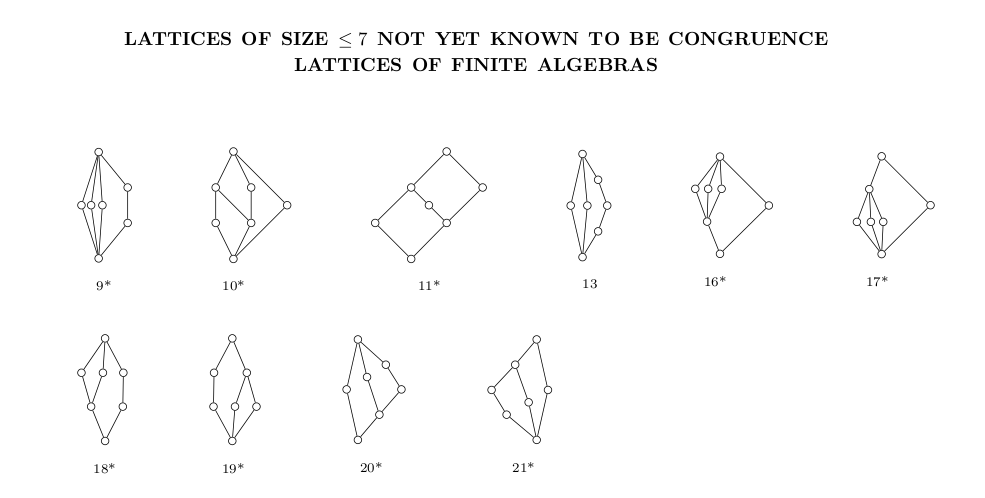
\includegraphics[height=2.3in]{figures/Sevens}
             \end{center}
             \hfill {\small {\it Figure courtesy of Peter Jipsen.}}
}  


\begin{frame}[label=knownresults,shrink=5]{
    Are all lattices with at most 7 elements representable?}

  \begin{columns}
    \begin{column}{0.2\textwidth}
      \begin{center}
        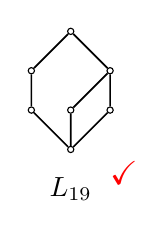
\begin{tikzpicture}[scale=.5]

          % L19
        \node (bottom) at (0,0)  [draw, circle, inner sep=\dotsize] {};
        \node (top) at (0,3)  [draw, circle, inner sep=\dotsize] {};
        \node (11) at (1,1)  [draw, circle, inner sep=\dotsize] {};
        \node (n11) at (-1,1)  [draw, circle, inner sep=\dotsize] {};
        \node (12) at (1,2)  [draw, circle, inner sep=\dotsize] {};
        \node (n12) at (-1,2)  [draw, circle, inner sep=\dotsize] {};
        \node (01) at (0,1)  [draw, circle, inner sep=\dotsize] {};

        \draw[semithick] (bottom) to (11) to (12) to (top) to (n12) to (n11) to (bottom) to (01) to (12);

          \draw (0,-1) node {$L_{19}$};
          \visible<2->{ {\color{red}\draw[font=\large] (1,-.6) node{$\text{\rlap{$\checkmark$}}$ };}
            %\draw[font=\large] (2.5,-.6) node { {\footnotesize Jipsen}};
          }

        \end{tikzpicture}
      \end{center}
    \end{column}
    \begin{column}{0.2\textwidth}
      \begin{center}
        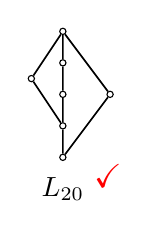
\begin{tikzpicture}[scale=.4]
          % L20
      \foreach \j in {0,...,4}
      {
        \node (0\j) at (0,\j)  [draw, circle, inner sep=\dotsize] {};
      }
      \node (152) at (1.5,2)  [draw, circle, inner sep=\dotsize] {};
      \node (n125) at (-1,2.5)  [draw, circle, inner sep=\dotsize] {};
      \draw[semithick] (01) to (02) to (03) to (04) to (n125) to (01) to (00) to (152) to (04);

          \draw (0,-1) node {$L_{20}$};
          \visible<2->{        {\color{red}\draw[font=\large] (1,-.6) node{$\text{\rlap{$\checkmark$}}$ };}
            %\draw[font=\large] (3,-.6) node { {\footnotesize Jipsen}};
          }
        \end{tikzpicture}
      \end{center}
    \end{column}
  \end{columns}

  \begin{columns}
    \begin{column}{0.2\textwidth}
      \begin{center}
        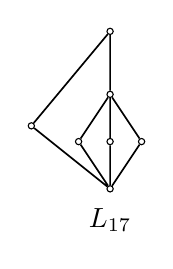
\begin{tikzpicture}[scale=.4]

          
        \node (bottom) at (0,0)  [draw, circle, inner sep=\dotsize] {};
        \node (top) at (0,5)  [draw, circle, inner sep=\dotsize] {};
        \node (n115) at (-1,1.5)  [draw, circle, inner sep=\dotsize] {};
        \node (015) at (0,1.5)  [draw, circle, inner sep=\dotsize] {};
        \node (115) at (1,1.5)  [draw, circle, inner sep=\dotsize] {};
        \node (n252) at (-2.5,2)  [draw, circle, inner sep=\dotsize] {};
        \node (03) at (0,3)  [draw, circle, inner sep=\dotsize] {};
        \draw[semithick] 
        (bottom) to (n252) to (top)
        (bottom) to (n115) to (03) to (115) to
        (bottom) to (015) to (03) to (top);
       %\draw (-4.5,2.2) node {$L \cong$};



          \draw (0,-1) node {$L_{17}$};
        \end{tikzpicture}
      \end{center}
    \end{column}

    \begin{column}{0.2\textwidth}
      \begin{center}
        \begin{tikzpicture}[scale=.5]

          %\newcommand{\dotsize}{1};
\node[lat] (0) at (0,0) {};
\node[lat] (1) at (-0,1) {};
\node[lat] (2) at (1,2) {};
\node[lat] (3) at (-1,2) {};
\node[lat] (4) at (-0,2) {};
\node[lat] (5) at (-0,3) {};
\node[lat] (6) at (-0,4) {};
%\draw[font=\scriptsize] (0,-.5) node {[A4, (C2 x C2 x C2 x C2) : A5]};
%\draw[font=\scriptsize] (0,-1) node {SmallGroup(960,11358) Index 80};

\draw[semithick]
(0) to (1) to (4) to (5) to (6)
(0) to (2) to (6) to (3) to (0);


          \draw (0,-.6) node {$L_{13}$};

        \end{tikzpicture}
      \end{center}
    \end{column}

    \begin{column}{0.2\textwidth}
      \begin{center}
        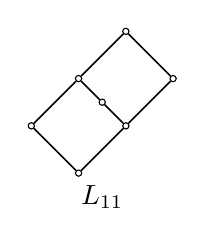
\begin{tikzpicture}[scale=.3]

          % L11 aka L3 
        \node (bottom) at (0,0)  [draw, circle, inner sep=\dotsize] {};
        \node (top) at (2,6)  [draw, circle, inner sep=\dotsize] {};
        \node (n22) at (-2,2)  [draw, circle, inner sep=\dotsize] {};
        \node (22) at (2,2)  [draw, circle, inner sep=\dotsize] {};
        \node (13) at (1,3)  [draw, circle, inner sep=\dotsize] {};
        \node (04) at (0,4)  [draw, circle, inner sep=\dotsize] {};
        \node (44) at (4,4)  [draw, circle, inner sep=\dotsize] {};

        \draw[semithick] (bottom) to (22) to (44) to (top) to (04) to (13) to (22)
        (bottom) to (n22) to (04);
  
          \draw (1,-1) node {$L_{11}$};
          %{$L_{11}$ {\small (aka $L_3$)}};

        \end{tikzpicture}
      \end{center}
    \end{column}

  \end{columns}


  \begin{columns}

    \begin{column}{0.2\textwidth}
      \begin{center}
        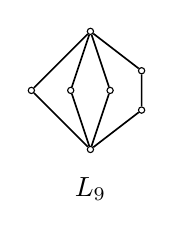
\begin{tikzpicture}[scale=.5]

          %% ``L9'' is the pentegon with two extra wings.
      \foreach \j in {0,3} 
      { \node (7\j) at (6.5,\j)  [draw, circle, inner sep=\dotsize] {};}
      \node (71) at (7,1.5)  [draw, circle, inner sep=\dotsize] {};
      \node (61) at (6,1.5)  [draw, circle, inner sep=\dotsize] {};
      \node (51) at (5,1.5)  [draw, circle, inner sep=\dotsize] {};
      \foreach \j in {1,2} 
      { \node (8\j) at (7.8,\j)  [draw, circle, inner sep=\dotsize] {};}
      \draw[semithick] (70) to (51) to (73) to (61) to (70) to (71) to (73) to
      (82) to (81) to (70);
      

          \draw (6.5,-1) node {$L_{9}$};

        \end{tikzpicture}
      \end{center}
    \end{column}


    \begin{column}{0.2\textwidth}
      \begin{center}
        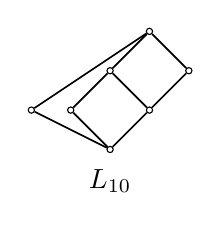
\begin{tikzpicture}[scale=.5]

          %%  The elusive winged-2x3 %%
      \node (01) at (0,1)  [draw, circle, inner sep=\dotsize] {};
      \foreach \j in {0,2} 
      { \node (1\j) at (1,\j)  [draw, circle, inner sep=\dotsize] {};}

      \foreach \j in {1,3} 
      { \node (2\j) at (2,\j)  [draw, circle, inner sep=\dotsize] {};}
      { \node (32) at (3,2)  [draw, circle, inner sep=\dotsize] {};}
      \draw[semithick] (10) to (01) to (12) to (23) to (32) to (21) to (10) (21) to (12);
      { \node (m11) at (-1,1)  [draw, circle, inner sep=\dotsize] {};}
      \draw[semithick] (10) to (m11) to (23);


          \draw (1,-.8) node {$L_{10}$};

        \end{tikzpicture}
      \end{center}
    \end{column}
  \end{columns}
\end{frame}


\begin{frame}[label=knownresults,shrink=5]{Finding representations...}
  \framesubtitle{...as intervals in subgroup lattices}

  \begin{columns}
    \begin{column}{0.2\textwidth}
      \begin{center}
        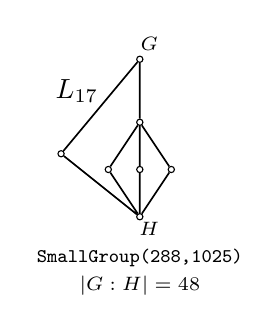
\begin{tikzpicture}[scale=.4]

          
        \node (bottom) at (0,0)  [draw, circle, inner sep=\dotsize] {};
        \node (top) at (0,5)  [draw, circle, inner sep=\dotsize] {};
        \node (n115) at (-1,1.5)  [draw, circle, inner sep=\dotsize] {};
        \node (015) at (0,1.5)  [draw, circle, inner sep=\dotsize] {};
        \node (115) at (1,1.5)  [draw, circle, inner sep=\dotsize] {};
        \node (n252) at (-2.5,2)  [draw, circle, inner sep=\dotsize] {};
        \node (03) at (0,3)  [draw, circle, inner sep=\dotsize] {};
        \draw[semithick] 
        (bottom) to (n252) to (top)
        (bottom) to (n115) to (03) to (115) to
        (bottom) to (015) to (03) to (top);
       %\draw (-4.5,2.2) node {$L \cong$};




          \draw (-2,4) node {$L_{17}$};
          \uncover<2->{
            \draw[font=\scriptsize] (0.3,5.5) node {$G$};
            \draw[font=\scriptsize] (0.3,-.4) node { $H$};
            \draw[font=\scriptsize] (0,-1.3) node {{\tt SmallGroup(288,1025)}};
            \draw[font=\scriptsize] (0,-2.2) node { $|G:H|=48$};
          }

        \end{tikzpicture}
      \end{center}
    \end{column}

    \uncover<2->{
      \begin{column}{0.6\textwidth}
        \begin{itemize}
        \item 
          The group $G = (A_4 \times A_4) \rtimes C_2$ has a subgroup $H\cong S_3$ such
          that $\lb H,G \rb\cong L_{17}$.
          \vskip10pt
        \item<2-> ...so the dual $L_{16}$ is also representable.
          %% \\[8pt]
          %%   {\small $L_{16}$ can be embedded above diagonal of the direct power of
          %%     a simple group,
          %%     \[L_{16} \hookrightarrow \lb D,S^{48} \rb \cong \Eq(48)^{dual}.\]  
          %%     Add the group operations $G$ which closed $L_{17}$, and $L_{16}$ appears as an upper interval in $S^{48} \rtimes G$.}

        \end{itemize}
      \end{column}
    }
  \end{columns}

  \begin{columns}
    \begin{column}{0.3\textwidth}
      \begin{center}
        \begin{tikzpicture}[scale=.5]

          %\newcommand{\dotsize}{1};
\node[lat] (0) at (0,0) {};
\node[lat] (1) at (-0,1) {};
\node[lat] (2) at (1,2) {};
\node[lat] (3) at (-1,2) {};
\node[lat] (4) at (-0,2) {};
\node[lat] (5) at (-0,3) {};
\node[lat] (6) at (-0,4) {};
%\draw[font=\scriptsize] (0,-.5) node {[A4, (C2 x C2 x C2 x C2) : A5]};
%\draw[font=\scriptsize] (0,-1) node {SmallGroup(960,11358) Index 80};

\draw[semithick]
(0) to (1) to (4) to (5) to (6)
(0) to (2) to (6) to (3) to (0);



          \draw (-1.5,3) node {$L_{13}$};
          \uncover<3->{
            \draw[font=\scriptsize] (0.3,4.3) node {$G$};
            \draw[font=\scriptsize] (0.3,-.4) node { $H$};
            \draw[font=\scriptsize] (0,-1) node {{\tt SmallGroup(960,11358)}};
            \draw[font=\scriptsize] (0,-1.7) node {$|G:H|=80$};
          }
        \end{tikzpicture}
      \end{center}
    \end{column}
    \begin{column}{0.65\textwidth}
      \begin{itemize}
      \item<3-> 
        The group $G = (C_2 \times C_2 \times C_2 \times C_2) \rtimes A_5$
        has a subgroup $H\cong A_4$ such that $\lb H,G \rb\cong L_{13}$.
      \end{itemize}
    \end{column}
  \end{columns}


\end{frame}


%\begin{frame}[label=knownresults,shrink=5]{Finding representations...}
\begin{frame}[label=knownresultsdrop,shrink=5]{
    Are all lattices with at most 7 elements representable?}

  \begin{columns}
    \begin{column}{0.2\textwidth}
      \begin{center}
        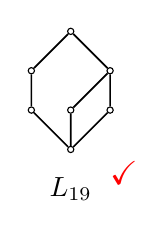
\begin{tikzpicture}[scale=.5]

          % L19
        \node (bottom) at (0,0)  [draw, circle, inner sep=\dotsize] {};
        \node (top) at (0,3)  [draw, circle, inner sep=\dotsize] {};
        \node (11) at (1,1)  [draw, circle, inner sep=\dotsize] {};
        \node (n11) at (-1,1)  [draw, circle, inner sep=\dotsize] {};
        \node (12) at (1,2)  [draw, circle, inner sep=\dotsize] {};
        \node (n12) at (-1,2)  [draw, circle, inner sep=\dotsize] {};
        \node (01) at (0,1)  [draw, circle, inner sep=\dotsize] {};

        \draw[semithick] (bottom) to (11) to (12) to (top) to (n12) to (n11) to (bottom) to (01) to (12);

          \draw (0,-1) node {$L_{19}$};
                {\color{red}\draw[font=\large] (1,-.6) node{$\text{\rlap{$\checkmark$}}$ };}
                %\draw[font=\large] (2.5,-.6) node { {\footnotesize Jipsen}};

        \end{tikzpicture}
      \end{center}
    \end{column}
    \begin{column}{0.2\textwidth}
      \begin{center}
        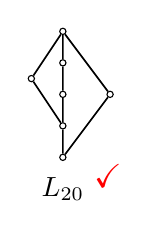
\begin{tikzpicture}[scale=.4]
          % L20
      \foreach \j in {0,...,4}
      {
        \node (0\j) at (0,\j)  [draw, circle, inner sep=\dotsize] {};
      }
      \node (152) at (1.5,2)  [draw, circle, inner sep=\dotsize] {};
      \node (n125) at (-1,2.5)  [draw, circle, inner sep=\dotsize] {};
      \draw[semithick] (01) to (02) to (03) to (04) to (n125) to (01) to (00) to (152) to (04);

          \draw (0,-1) node {$L_{20}$};
                {\color{red}\draw[font=\large] (1,-.6) node{$\text{\rlap{$\checkmark$}}$ };}
                %\draw[font=\large] (3,-.6) node { {\footnotesize Jipsen}};
        \end{tikzpicture}
      \end{center}
    \end{column}
  \end{columns}

  \begin{columns}
    \begin{column}{0.2\textwidth}
      \begin{center}
        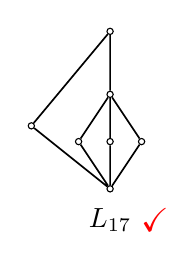
\begin{tikzpicture}[scale=.4]

          
        \node (bottom) at (0,0)  [draw, circle, inner sep=\dotsize] {};
        \node (top) at (0,5)  [draw, circle, inner sep=\dotsize] {};
        \node (n115) at (-1,1.5)  [draw, circle, inner sep=\dotsize] {};
        \node (015) at (0,1.5)  [draw, circle, inner sep=\dotsize] {};
        \node (115) at (1,1.5)  [draw, circle, inner sep=\dotsize] {};
        \node (n252) at (-2.5,2)  [draw, circle, inner sep=\dotsize] {};
        \node (03) at (0,3)  [draw, circle, inner sep=\dotsize] {};
        \draw[semithick] 
        (bottom) to (n252) to (top)
        (bottom) to (n115) to (03) to (115) to
        (bottom) to (015) to (03) to (top);
       %\draw (-4.5,2.2) node {$L \cong$};



          \draw (0,-1) node {$L_{17}$};
                {\color{red}\draw[font=\large] (1,-1) node{$\text{\rlap{$\checkmark$}}$ };}


        \end{tikzpicture}
      \end{center}
    \end{column}

    \begin{column}{0.2\textwidth}
      \begin{center}
        \begin{tikzpicture}[scale=.5]

          %\newcommand{\dotsize}{1};
\node[lat] (0) at (0,0) {};
\node[lat] (1) at (-0,1) {};
\node[lat] (2) at (1,2) {};
\node[lat] (3) at (-1,2) {};
\node[lat] (4) at (-0,2) {};
\node[lat] (5) at (-0,3) {};
\node[lat] (6) at (-0,4) {};
%\draw[font=\scriptsize] (0,-.5) node {[A4, (C2 x C2 x C2 x C2) : A5]};
%\draw[font=\scriptsize] (0,-1) node {SmallGroup(960,11358) Index 80};

\draw[semithick]
(0) to (1) to (4) to (5) to (6)
(0) to (2) to (6) to (3) to (0);


          \draw (0,-.6) node {$L_{13}$};
                {\color{red}\draw[font=\large] (1,-.6) node{$\text{\rlap{$\checkmark$}}$ };}

        \end{tikzpicture}
      \end{center}
    \end{column}

    \begin{column}{0.2\textwidth}
      \begin{center}
        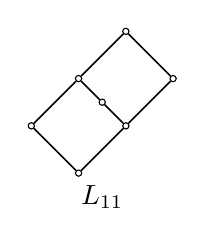
\begin{tikzpicture}[scale=.3]

          % L11 aka L3 
        \node (bottom) at (0,0)  [draw, circle, inner sep=\dotsize] {};
        \node (top) at (2,6)  [draw, circle, inner sep=\dotsize] {};
        \node (n22) at (-2,2)  [draw, circle, inner sep=\dotsize] {};
        \node (22) at (2,2)  [draw, circle, inner sep=\dotsize] {};
        \node (13) at (1,3)  [draw, circle, inner sep=\dotsize] {};
        \node (04) at (0,4)  [draw, circle, inner sep=\dotsize] {};
        \node (44) at (4,4)  [draw, circle, inner sep=\dotsize] {};

        \draw[semithick] (bottom) to (22) to (44) to (top) to (04) to (13) to (22)
        (bottom) to (n22) to (04);
  \draw (1,-1) node {$L_{11}$};

        \end{tikzpicture}
      \end{center}
    \end{column}

  \end{columns}

  \begin{columns}

    \begin{column}{0.2\textwidth}
      \begin{center}
        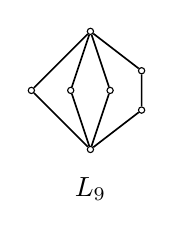
\begin{tikzpicture}[scale=.5]

          %% ``L9'' is the pentegon with two extra wings.
      \foreach \j in {0,3} 
      { \node (7\j) at (6.5,\j)  [draw, circle, inner sep=\dotsize] {};}
      \node (71) at (7,1.5)  [draw, circle, inner sep=\dotsize] {};
      \node (61) at (6,1.5)  [draw, circle, inner sep=\dotsize] {};
      \node (51) at (5,1.5)  [draw, circle, inner sep=\dotsize] {};
      \foreach \j in {1,2} 
      { \node (8\j) at (7.8,\j)  [draw, circle, inner sep=\dotsize] {};}
      \draw[semithick] (70) to (51) to (73) to (61) to (70) to (71) to (73) to
      (82) to (81) to (70);
      

          \draw (6.5,-1) node {$L_{9}$};

        \end{tikzpicture}
      \end{center}
    \end{column}


    \begin{column}{0.2\textwidth}
      \begin{center}
        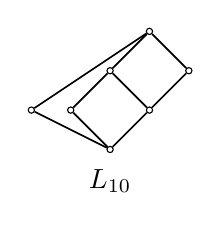
\begin{tikzpicture}[scale=.5]

          %%  The elusive winged-2x3 %%
      \node (01) at (0,1)  [draw, circle, inner sep=\dotsize] {};
      \foreach \j in {0,2} 
      { \node (1\j) at (1,\j)  [draw, circle, inner sep=\dotsize] {};}

      \foreach \j in {1,3} 
      { \node (2\j) at (2,\j)  [draw, circle, inner sep=\dotsize] {};}
      { \node (32) at (3,2)  [draw, circle, inner sep=\dotsize] {};}
      \draw[semithick] (10) to (01) to (12) to (23) to (32) to (21) to (10) (21) to (12);
      { \node (m11) at (-1,1)  [draw, circle, inner sep=\dotsize] {};}
      \draw[semithick] (10) to (m11) to (23);


          \draw (1,-.8) node {$L_{10}$};

        \end{tikzpicture}
      \end{center}
    \end{column}
  \end{columns}
\end{frame}



\begin{frame}[label=knownresults,shrink=5]{Finding representations...}
  \framesubtitle{...using subgroup lattice intervals and the filter+ideal lemma.}

  %\uncover<2->{
  \begin{columns}
    \begin{column}{0.2\textwidth}
      \begin{center}
        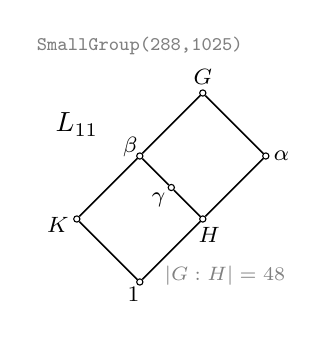
\begin{tikzpicture}[scale=.4]
          % L11 aka L3 
        \node (bottom) at (0,0)  [draw, circle, inner sep=\dotsize] {};
        \node (top) at (2,6)  [draw, circle, inner sep=\dotsize] {};
        \node (n22) at (-2,2)  [draw, circle, inner sep=\dotsize] {};
        \node (22) at (2,2)  [draw, circle, inner sep=\dotsize] {};
        \node (13) at (1,3)  [draw, circle, inner sep=\dotsize] {};
        \node (04) at (0,4)  [draw, circle, inner sep=\dotsize] {};
        \node (44) at (4,4)  [draw, circle, inner sep=\dotsize] {};

        \draw[semithick] (bottom) to (22) to (44) to (top) to (04) to (13) to (22)
        (bottom) to (n22) to (04);
;
          \draw (-2,5) node {$L_{11}$};
          \uncover<2->{
            \draw[font=\footnotesize] 
            (2,6.5) node {$G$} (2.2,1.5) node {$H$} (-.2,-.4) node {$1$}
            (4.5,4) node {$\alpha$} (-.3,4.3) node {$\beta$} (.6,2.6) node {$\gamma$};
                 {\color{gray} \draw[font=\scriptsize] (0,7.5) node {{\tt SmallGroup(288,1025)}};}
                 {\color{gray} \draw[font=\scriptsize] (2.7,.2) node {$|G:H|=48$};}
          }
          \uncover<3->{
            \draw[font=\footnotesize]  (-2.6,1.8) node {$K$};
          }
        \end{tikzpicture}
      \end{center}
    \end{column}
    \begin{column}{0.6\textwidth}
      \vskip1cm
      \begin{itemize}
      \item<2-> 
        Let $G=(A_4 \times A_4) \rtimes C_2$. %\hskip6pt ($|G| = 216$).
      \item<2-> $G$ has a subgroup $H \cong C_6$ with $\lb H, G \rb \cong N_5$. \hskip6pt %($|G:H| = 36$).
      \item<2-> Let $\lb H, G \rb = \{H, \alpha, \beta, \gamma, G\} \cong N_5$.\vskip6pt
      \item<3-> $\Sub(G)$ is a congruence lattice, so
        if there exists a subgroup $K \succ 1$, below $\beta$ and not below $\gamma$, 
        then \[L_{11} \cong K^\downarrow \cup H^\uparrow.\]
      \end{itemize}
    \end{column}
  \end{columns}
  %}

  \uncover<4->{
    \begin{columns}
      \begin{column}{0.2\textwidth}
        \begin{center}
          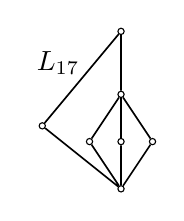
\begin{tikzpicture}[scale=.4]
            
        \node (bottom) at (0,0)  [draw, circle, inner sep=\dotsize] {};
        \node (top) at (0,5)  [draw, circle, inner sep=\dotsize] {};
        \node (n115) at (-1,1.5)  [draw, circle, inner sep=\dotsize] {};
        \node (015) at (0,1.5)  [draw, circle, inner sep=\dotsize] {};
        \node (115) at (1,1.5)  [draw, circle, inner sep=\dotsize] {};
        \node (n252) at (-2.5,2)  [draw, circle, inner sep=\dotsize] {};
        \node (03) at (0,3)  [draw, circle, inner sep=\dotsize] {};
        \draw[semithick] 
        (bottom) to (n252) to (top)
        (bottom) to (n115) to (03) to (115) to
        (bottom) to (015) to (03) to (top);
       %\draw (-4.5,2.2) node {$L \cong$};


;
            \draw (-2,4) node {$L_{17}$};
          \end{tikzpicture}
        \end{center}
      \end{column}
      \begin{column}{0.3\textwidth}
        \begin{center}
          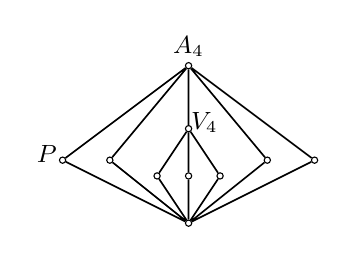
\begin{tikzpicture}[scale=.4]
                    \node (bottom) at (0,0)  [draw, circle, inner sep=\dotsize] {};
        \node (top) at (0,5)  [draw, circle, inner sep=\dotsize] {};
        \node (n115) at (-1,1.5)  [draw, circle, inner sep=\dotsize] {};
        \node (015) at (0,1.5)  [draw, circle, inner sep=\dotsize] {};
        \node (115) at (1,1.5)  [draw, circle, inner sep=\dotsize] {};
        \node (n252) at (-2.5,2)  [draw, circle, inner sep=\dotsize] {};
        \node (252) at (2.5,2)  [draw, circle, inner sep=\dotsize] {};
        \node (n42) at (-4,2)  [draw, circle, inner sep=\dotsize] {};
        \node (42) at (4,2)  [draw, circle, inner sep=\dotsize] {};
        \node (03) at (0,3)  [draw, circle, inner sep=\dotsize] {};
        \draw[semithick] 
        (bottom) to (42) to (top) to (n42) to 
        (bottom) to (n252) to (top) to (252) to 
        (bottom) to (n115) to (03) to (115) to
        (bottom) to (015) to (03) to (top);

            \draw[font=\small] (0,5.6) node {$A_4$};
            \draw[font=\small] (.5,3.2) node {$V_4$};
            \draw[font=\small] (-4.5,2.2) node {$P$};
          \end{tikzpicture}
        \end{center}
      \end{column}
      \begin{column}{0.45\textwidth}
        \begin{itemize}
        \item $\Sub(A_4)$ is a congruence lattice 
          {\footnotesize (of $A_4$ acting regularly on itself).}\vskip6pt
        \item Therefore, 
          \[L_{17} \cong V_4^\downarrow \cup P^\uparrow\]
          is a congruence lattice.
        \end{itemize}
      \end{column}
  }

    \end{columns}

\end{frame}


\begin{frame}[label=knownresults,shrink=5]{
    Are all lattices with at most 7 elements representable?}
  \begin{columns}
    \begin{column}{0.2\textwidth}
      \begin{center}
        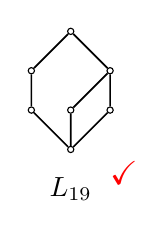
\begin{tikzpicture}[scale=.5]

          % L19
        \node (bottom) at (0,0)  [draw, circle, inner sep=\dotsize] {};
        \node (top) at (0,3)  [draw, circle, inner sep=\dotsize] {};
        \node (11) at (1,1)  [draw, circle, inner sep=\dotsize] {};
        \node (n11) at (-1,1)  [draw, circle, inner sep=\dotsize] {};
        \node (12) at (1,2)  [draw, circle, inner sep=\dotsize] {};
        \node (n12) at (-1,2)  [draw, circle, inner sep=\dotsize] {};
        \node (01) at (0,1)  [draw, circle, inner sep=\dotsize] {};

        \draw[semithick] (bottom) to (11) to (12) to (top) to (n12) to (n11) to (bottom) to (01) to (12);

          \draw (0,-1) node {$L_{19}$};
                {\color{red}\draw[font=\large] (1,-.6) node{$\text{\rlap{$\checkmark$}}$ };}
                %\draw[font=\footnotesize] (2.5,-.6) node { Jipsen};

        \end{tikzpicture}
      \end{center}
    \end{column}
    \begin{column}{0.2\textwidth}
      \begin{center}
        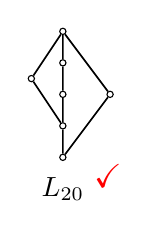
\begin{tikzpicture}[scale=.4]
          % L20
      \foreach \j in {0,...,4}
      {
        \node (0\j) at (0,\j)  [draw, circle, inner sep=\dotsize] {};
      }
      \node (152) at (1.5,2)  [draw, circle, inner sep=\dotsize] {};
      \node (n125) at (-1,2.5)  [draw, circle, inner sep=\dotsize] {};
      \draw[semithick] (01) to (02) to (03) to (04) to (n125) to (01) to (00) to (152) to (04);

          \draw (0,-1) node {$L_{20}$};
                {\color{red}\draw[font=\large] (1,-.6) node{$\text{\rlap{$\checkmark$}}$ };}
                %\draw[font=\footnotesize] (3,-.6) node { Jipsen};
        \end{tikzpicture}
      \end{center}
    \end{column}
  \end{columns}

  \begin{columns}
    \begin{column}{0.2\textwidth}
      \begin{center}
        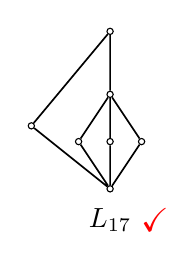
\begin{tikzpicture}[scale=.4]

          
        \node (bottom) at (0,0)  [draw, circle, inner sep=\dotsize] {};
        \node (top) at (0,5)  [draw, circle, inner sep=\dotsize] {};
        \node (n115) at (-1,1.5)  [draw, circle, inner sep=\dotsize] {};
        \node (015) at (0,1.5)  [draw, circle, inner sep=\dotsize] {};
        \node (115) at (1,1.5)  [draw, circle, inner sep=\dotsize] {};
        \node (n252) at (-2.5,2)  [draw, circle, inner sep=\dotsize] {};
        \node (03) at (0,3)  [draw, circle, inner sep=\dotsize] {};
        \draw[semithick] 
        (bottom) to (n252) to (top)
        (bottom) to (n115) to (03) to (115) to
        (bottom) to (015) to (03) to (top);
       %\draw (-4.5,2.2) node {$L \cong$};



          \draw (0,-1) node {$L_{17}$};
                {\color{red}\draw[font=\large] (1,-1) node{$\text{\rlap{$\checkmark$}}$ };}

        \end{tikzpicture}
      \end{center}
    \end{column}

    \begin{column}{0.2\textwidth}
      \begin{center}
        \begin{tikzpicture}[scale=.5]

          %\newcommand{\dotsize}{1};
\node[lat] (0) at (0,0) {};
\node[lat] (1) at (-0,1) {};
\node[lat] (2) at (1,2) {};
\node[lat] (3) at (-1,2) {};
\node[lat] (4) at (-0,2) {};
\node[lat] (5) at (-0,3) {};
\node[lat] (6) at (-0,4) {};
%\draw[font=\scriptsize] (0,-.5) node {[A4, (C2 x C2 x C2 x C2) : A5]};
%\draw[font=\scriptsize] (0,-1) node {SmallGroup(960,11358) Index 80};

\draw[semithick]
(0) to (1) to (4) to (5) to (6)
(0) to (2) to (6) to (3) to (0);


          \draw (0,-.6) node {$L_{13}$};
                {\color{red}\draw[font=\large] (1,-.6) node{$\text{\rlap{$\checkmark$}}$ };}

        \end{tikzpicture}
      \end{center}
    \end{column}

    \begin{column}{0.2\textwidth}
      \begin{center}
        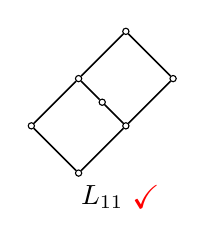
\begin{tikzpicture}[scale=.3]

          % L11 aka L3 
        \node (bottom) at (0,0)  [draw, circle, inner sep=\dotsize] {};
        \node (top) at (2,6)  [draw, circle, inner sep=\dotsize] {};
        \node (n22) at (-2,2)  [draw, circle, inner sep=\dotsize] {};
        \node (22) at (2,2)  [draw, circle, inner sep=\dotsize] {};
        \node (13) at (1,3)  [draw, circle, inner sep=\dotsize] {};
        \node (04) at (0,4)  [draw, circle, inner sep=\dotsize] {};
        \node (44) at (4,4)  [draw, circle, inner sep=\dotsize] {};

        \draw[semithick] (bottom) to (22) to (44) to (top) to (04) to (13) to (22)
        (bottom) to (n22) to (04);
  \draw (1,-1) node {$L_{11}$};
                {\color{red}\draw[font=\large] (2.3,-1) node { $\text{\rlap{$\checkmark$}}$};}

        \end{tikzpicture}
      \end{center}
    \end{column}

  \end{columns}


  \begin{columns}

    \begin{column}{0.2\textwidth}
      \begin{center}
        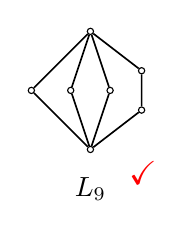
\begin{tikzpicture}[scale=.5]

          %% ``L9'' is the pentegon with two extra wings.
      \foreach \j in {0,3} 
      { \node (7\j) at (6.5,\j)  [draw, circle, inner sep=\dotsize] {};}
      \node (71) at (7,1.5)  [draw, circle, inner sep=\dotsize] {};
      \node (61) at (6,1.5)  [draw, circle, inner sep=\dotsize] {};
      \node (51) at (5,1.5)  [draw, circle, inner sep=\dotsize] {};
      \foreach \j in {1,2} 
      { \node (8\j) at (7.8,\j)  [draw, circle, inner sep=\dotsize] {};}
      \draw[semithick] (70) to (51) to (73) to (61) to (70) to (71) to (73) to
      (82) to (81) to (70);
      

          \draw (6.5,-1) node {$L_{9}$};
          \uncover<2->{
            {\color{red}\draw[font=\large] (7.5,-.6) node{$\text{\rlap{$\checkmark$}}$ };}
            %\draw[font=\large] (9.3,-.6) node { {\footnotesize Freese}};
          }
        \end{tikzpicture}
      \end{center}
    \end{column}


    \begin{column}{0.2\textwidth}
      \begin{center}
        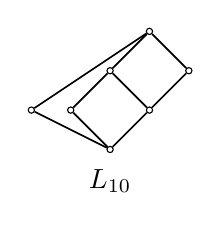
\begin{tikzpicture}[scale=.5]

          %%  The elusive winged-2x3 %%
      \node (01) at (0,1)  [draw, circle, inner sep=\dotsize] {};
      \foreach \j in {0,2} 
      { \node (1\j) at (1,\j)  [draw, circle, inner sep=\dotsize] {};}

      \foreach \j in {1,3} 
      { \node (2\j) at (2,\j)  [draw, circle, inner sep=\dotsize] {};}
      { \node (32) at (3,2)  [draw, circle, inner sep=\dotsize] {};}
      \draw[semithick] (10) to (01) to (12) to (23) to (32) to (21) to (10) (21) to (12);
      { \node (m11) at (-1,1)  [draw, circle, inner sep=\dotsize] {};}
      \draw[semithick] (10) to (m11) to (23);



%          \visible<3>{\node (18) at (1,1.3)  [draw, circle, red, inner sep=25pt] {};} 

          \draw (1,-.8) node {$L_{10}$};
        \end{tikzpicture}
      \end{center}
    \end{column}
  \end{columns}
\end{frame}




%% \begin{frame}[label=elusive,shrink=5]{The Elusive Seven Element Lattice}
%%   \begin{columns}
%%     \begin{column}{0.2\textwidth}
%%       \begin{center}
%%         \begin{tikzpicture}[scale=.5]

%%           % L19
        \node (bottom) at (0,0)  [draw, circle, inner sep=\dotsize] {};
        \node (top) at (0,3)  [draw, circle, inner sep=\dotsize] {};
        \node (11) at (1,1)  [draw, circle, inner sep=\dotsize] {};
        \node (n11) at (-1,1)  [draw, circle, inner sep=\dotsize] {};
        \node (12) at (1,2)  [draw, circle, inner sep=\dotsize] {};
        \node (n12) at (-1,2)  [draw, circle, inner sep=\dotsize] {};
        \node (01) at (0,1)  [draw, circle, inner sep=\dotsize] {};

        \draw[semithick] (bottom) to (11) to (12) to (top) to (n12) to (n11) to (bottom) to (01) to (12);

%%           \draw (0,-1) node {$L_{19}$};
%%                 {\color{red}\draw[font=\large] (1,-.6) node{$\text{\rlap{$\checkmark$}}$ };}
%%                 %\draw[font=\footnotesize] (2.5,-.6) node { Jipsen};

%%         \end{tikzpicture}
%%       \end{center}
%%     \end{column}
%%     \begin{column}{0.2\textwidth}
%%       \begin{center}
%%         \begin{tikzpicture}[scale=.4]
%%           % L20
      \foreach \j in {0,...,4}
      {
        \node (0\j) at (0,\j)  [draw, circle, inner sep=\dotsize] {};
      }
      \node (152) at (1.5,2)  [draw, circle, inner sep=\dotsize] {};
      \node (n125) at (-1,2.5)  [draw, circle, inner sep=\dotsize] {};
      \draw[semithick] (01) to (02) to (03) to (04) to (n125) to (01) to (00) to (152) to (04);

%%           \draw (0,-1) node {$L_{20}$};
%%                 {\color{red}\draw[font=\large] (1,-.6) node{$\text{\rlap{$\checkmark$}}$ };}
%%                 %\draw[font=\footnotesize] (3,-.6) node { Jipsen};
%%         \end{tikzpicture}
%%       \end{center}
%%     \end{column}
%%   \end{columns}

%%   \begin{columns}
%%     \begin{column}{0.2\textwidth}
%%       \begin{center}
%%         \begin{tikzpicture}[scale=.4]

%%           
        \node (bottom) at (0,0)  [draw, circle, inner sep=\dotsize] {};
        \node (top) at (0,5)  [draw, circle, inner sep=\dotsize] {};
        \node (n115) at (-1,1.5)  [draw, circle, inner sep=\dotsize] {};
        \node (015) at (0,1.5)  [draw, circle, inner sep=\dotsize] {};
        \node (115) at (1,1.5)  [draw, circle, inner sep=\dotsize] {};
        \node (n252) at (-2.5,2)  [draw, circle, inner sep=\dotsize] {};
        \node (03) at (0,3)  [draw, circle, inner sep=\dotsize] {};
        \draw[semithick] 
        (bottom) to (n252) to (top)
        (bottom) to (n115) to (03) to (115) to
        (bottom) to (015) to (03) to (top);
       %\draw (-4.5,2.2) node {$L \cong$};



%%           \draw (0,-1) node {$L_{17}$};
%%                 {\color{red}\draw[font=\large] (1,-1) node{$\text{\rlap{$\checkmark$}}$ };}

%%         \end{tikzpicture}
%%       \end{center}
%%     \end{column}

%%     \begin{column}{0.2\textwidth}
%%       \begin{center}
%%         \begin{tikzpicture}[scale=.5]

%%           %\newcommand{\dotsize}{1};
\node[lat] (0) at (0,0) {};
\node[lat] (1) at (-0,1) {};
\node[lat] (2) at (1,2) {};
\node[lat] (3) at (-1,2) {};
\node[lat] (4) at (-0,2) {};
\node[lat] (5) at (-0,3) {};
\node[lat] (6) at (-0,4) {};
%\draw[font=\scriptsize] (0,-.5) node {[A4, (C2 x C2 x C2 x C2) : A5]};
%\draw[font=\scriptsize] (0,-1) node {SmallGroup(960,11358) Index 80};

\draw[semithick]
(0) to (1) to (4) to (5) to (6)
(0) to (2) to (6) to (3) to (0);


%%           \draw (0,-.6) node {$L_{13}$};
%%                 {\color{red}\draw[font=\large] (1,-.6) node{$\text{\rlap{$\checkmark$}}$ };}

%%         \end{tikzpicture}
%%       \end{center}
%%     \end{column}

%%     \begin{column}{0.2\textwidth}
%%       \begin{center}
%%         \begin{tikzpicture}[scale=.3]

%%           % L11 aka L3 
        \node (bottom) at (0,0)  [draw, circle, inner sep=\dotsize] {};
        \node (top) at (2,6)  [draw, circle, inner sep=\dotsize] {};
        \node (n22) at (-2,2)  [draw, circle, inner sep=\dotsize] {};
        \node (22) at (2,2)  [draw, circle, inner sep=\dotsize] {};
        \node (13) at (1,3)  [draw, circle, inner sep=\dotsize] {};
        \node (04) at (0,4)  [draw, circle, inner sep=\dotsize] {};
        \node (44) at (4,4)  [draw, circle, inner sep=\dotsize] {};

        \draw[semithick] (bottom) to (22) to (44) to (top) to (04) to (13) to (22)
        (bottom) to (n22) to (04);
  \draw (1,-1) node {$L_{11}$};
%%                 {\color{red}\draw[font=\large] (2.3,-1) node { $\text{\rlap{$\checkmark$}}$};}

%%         \end{tikzpicture}
%%       \end{center}
%%     \end{column}

%%   \end{columns}


%%   \begin{columns}

%%     \begin{column}{0.2\textwidth}
%%       \begin{center}
%%         \begin{tikzpicture}[scale=.5]

%%           %% ``L9'' is the pentegon with two extra wings.
      \foreach \j in {0,3} 
      { \node (7\j) at (6.5,\j)  [draw, circle, inner sep=\dotsize] {};}
      \node (71) at (7,1.5)  [draw, circle, inner sep=\dotsize] {};
      \node (61) at (6,1.5)  [draw, circle, inner sep=\dotsize] {};
      \node (51) at (5,1.5)  [draw, circle, inner sep=\dotsize] {};
      \foreach \j in {1,2} 
      { \node (8\j) at (7.8,\j)  [draw, circle, inner sep=\dotsize] {};}
      \draw[semithick] (70) to (51) to (73) to (61) to (70) to (71) to (73) to
      (82) to (81) to (70);
      

%%           \draw (6.5,-1) node {$L_{9}$};
%%             {\color{red}\draw[font=\large] (7.5,-.6) node{$\text{\rlap{$\checkmark$}}$ };}
%%             %\draw[font=\large] (9.3,-.6) node { {\footnotesize Freese}};
%%         \end{tikzpicture}
%%       \end{center}
%%     \end{column}


%%     \begin{column}{0.2\textwidth}
%%       \begin{center}
%%         \begin{tikzpicture}[scale=.5]

%%           %%  The elusive winged-2x3 %%
      \node (01) at (0,1)  [draw, circle, inner sep=\dotsize] {};
      \foreach \j in {0,2} 
      { \node (1\j) at (1,\j)  [draw, circle, inner sep=\dotsize] {};}

      \foreach \j in {1,3} 
      { \node (2\j) at (2,\j)  [draw, circle, inner sep=\dotsize] {};}
      { \node (32) at (3,2)  [draw, circle, inner sep=\dotsize] {};}
      \draw[semithick] (10) to (01) to (12) to (23) to (32) to (21) to (10) (21) to (12);
      { \node (m11) at (-1,1)  [draw, circle, inner sep=\dotsize] {};}
      \draw[semithick] (10) to (m11) to (23);



%%           %% \visible<2>{
%%             \node (18) at (1,1.3)  [draw, circle, red, inner sep=25pt] {};%% }

%%           \draw (1,-.8) node {$L_{10}$};
%%         \end{tikzpicture}
%%       \end{center}
%%     \end{column}
%%   \end{columns}
%% \end{frame}

%% \frame[label=MO,shrink=5]{
%%   \frametitle{Has anyone seen this lattice?}
%%   \begin{center}
%%     \includegraphics[height=2.8in]{figures/MOquestion201204}
%%   \end{center}
%% }  

%% \begin{frame}[fragile,shrink=5]{The Elusive Seven Element Lattice}
%% %\vskip5mm
%%   \begin{columns}
%%     \begin{column}{0.7\textwidth}
%%       \begin{itemize}
%%       \item  $L_{10}$ cannot be obtained using the overalgebra construction.
%%         \vskip3mm
%%       \item<2-> A minimal representation of $L_{10}$ must come from a transitive $G$-set.
%%         \vskip3mm
%%       \item<3-> If $\lb H,G \rb\cong L_{10}$ with $H$ core-free in $G$ then
%%         \vskip2mm
%%         \begin{itemize}
%%         \item $G$ is a non-solvable primitive permutation group.
%%           \vskip2mm
%%         \item $G$ is subdirectly irreducible.
%%         \end{itemize}
%%       \end{itemize}
%%     \end{column}
%%     \begin{column}{0.2\textwidth}
%%       \begin{center}
%%         \begin{tikzpicture}[scale=.5]

%%           %%  The elusive winged-2x3 %%
      \node (01) at (0,1)  [draw, circle, inner sep=\dotsize] {};
      \foreach \j in {0,2} 
      { \node (1\j) at (1,\j)  [draw, circle, inner sep=\dotsize] {};}

      \foreach \j in {1,3} 
      { \node (2\j) at (2,\j)  [draw, circle, inner sep=\dotsize] {};}
      { \node (32) at (3,2)  [draw, circle, inner sep=\dotsize] {};}
      \draw[semithick] (10) to (01) to (12) to (23) to (32) to (21) to (10) (21) to (12);
      { \node (m11) at (-1,1)  [draw, circle, inner sep=\dotsize] {};}
      \draw[semithick] (10) to (m11) to (23);



%%           \draw (1,-.8) node {$L_{10}$};
%%         \end{tikzpicture}
%%       \end{center}
%% %% \vskip5mm 
%% %%       \visible<4>{
%% %% \hskip-5mm          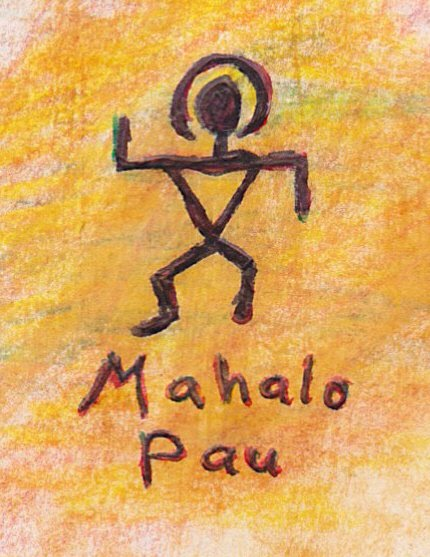
\includegraphics[height=2in]{figures/MahaloPau}
%% %%       }
%%     \end{column}
%%   \end{columns}
%% \end{frame}

\begin{frame}[fragile,label=freese,shrink=5]{Construction of an algebra $\bA$ with $\Con \bA \cong L_9$.}

  \begin{columns}
    \begin{column}{0.2\textwidth}

      \begin{center}
      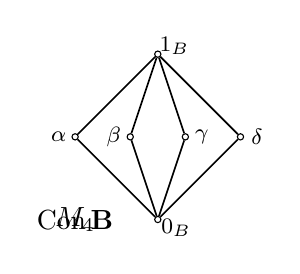
\begin{tikzpicture}[scale=.7]
                \node (250) at (2.5,0)  [draw, circle, inner sep=\dotsize] {};
        \node (253) at (2.5,3)  [draw, circle, inner sep=\dotsize] {};
        \foreach \i in {1,...,4} 
                 { 
                   \node (\i15) at (\i,1.5)  [draw, circle, inner sep=\dotsize] {};
                   \draw[semithick] (250) to (\i15) to (253);
                 }

        \uncover<2->{
          \draw[font=\footnotesize] 
          (0.7,1.5) node {$\alpha$} (1.7,1.5) node {$\beta$}
          (3.3,1.5) node {$\gamma$} (4.3,1.5) node {$\delta$}
          (2.8,3.15) node {$1_B$} (2.83,-.15) node {$0_B$};
        }
        \visible<1>{
          \draw  (1,0) node {$M_4$};}
        \visible<2->{
          \draw  (1,0) node {$\Con \bB$};}
      \end{tikzpicture}
      \end{center}

\vskip3mm

      \begin{center}
        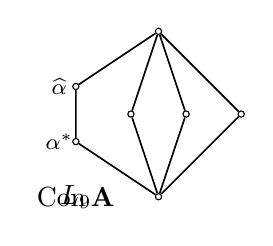
\begin{tikzpicture}[scale=.7]

                \node (70) at (6.5,0)  [draw, circle, inner sep=\dotsize] {};
      \node (71) at (7,1.5)  [draw, circle, inner sep=\dotsize] {};
      \node (73) at (6.5,3)  [draw, circle, inner sep=\dotsize] {};
      \node (61) at (6,1.5)  [draw, circle, inner sep=\dotsize] {};
      \node (51) at (5,1)  [draw, circle, inner sep=\dotsize] {};
      \node (52) at (5,2)  [draw, circle, inner sep=\dotsize] {};
      \node (81) at (8,1.5)  [draw, circle, inner sep=\dotsize] {};
      \draw[semithick] 
      (70) to (51) to (52) to (73)
      (70) to (61) to (73) 
      (70) to (71) to (73) 
      (70) to (81) to (73);

          \visible<1-3>{\draw  (5,0) node {$L_{9}$};}
          \visible<4->{\draw  (5,0) node {$\Con \bA$};}
          \visible<4->{\draw[font=\footnotesize] (4.7,2) node {$\widehat{\alpha}$} (4.7,1) node {$\alpha^*$};}

        \end{tikzpicture}
      \end{center}

    \end{column}


    \begin{column}{0.75\textwidth}
      \begin{enumerate}[Step 1]
      \item<2-> 
        Take a permutational algebra $\bB = \<B, F\>$ with congruence lattice $\Con\bB \cong M_4$.

        \vskip6pt
        
        \note{There are infinitely many, but apart from those involving 
          $S_3$, $C_3 \times C_3$, and $(C_3 \times C_3) \rtimes C_3$, they are quite
          large.  The next smallest G-set with $M_4$ congruence lattice that we
          know of comes from the group 
          $G = [ ( (C_3 \times C_3) \rtimes C_2 ) \times ( (C_3 \times C_3) \rtimes C_2 ) ] \rtimes C_2$
          acting on right cosets of $H \cong D_8$.  The index in this case is $|G:H| = 81$.
          (In \GAP, {\tt G:=SmallGroup(648,725)}.)}

        {\small
          \uncover<3->{\underline{Example:}
          \vskip4pt
          \begin{itemize}
%          \begin{itemize}[label=$\cdot$]
          \item
            Let $B = \{0, 1, \dots, 5\}$ index the elements of $S_3$ and
            consider the right regular action of $S_3$ on itself.
            \vskip5pt
          \item
            $g_0 = (0,4)(1,3)(2,5)$ and $g_1 = (0,1,2)(3,4,5)$ generate this
            action group, the image of $S_3 \hookrightarrow S_6$.
            \vskip5pt
          \item $\Con \<B , \{g_0, g_1\}\> \cong M_4$ with congruences
            \[
            \hskip-6mm            \alpha = | 0 1 2 | 3 4 5|, \; \beta = | 0 3 | 1 4 | 2 5 |, 
            \gamma = | 0 4|1 5| 2 3| , \; \delta = | 0 5|1 3| 2 4| .
            \]
          \end{itemize}}
        }

        \vskip6pt

\uncover<4->{
\hskip-10mm {\rmfamily {\bf Goal:} \emph{expand $\bB$ to an algebra $\bA$ that has
          $\alpha$ ``doubled'' in $\Con\bA$.}}}

        \vskip10pt

            \item<5-> Since $\alpha = \Cg^\bB(0,2)$, we let $A = B_0 \cup B_1 \cup B_2$ where
              \vskip-8pt
              \begin{align*}
                B_0 &= \{ {\color<5->{blue}0}, 1, {\color<5->{green}2}, 3, 4, 5\} = B\\
                B_1 &= \{{\color<5->{blue}0}, 6, 7, 8, 9, 10\}\\
                B_2 &= \{ 11, 12, {\color<5->{green}2}, 13, 14, 15\}.
              \end{align*}
            \item<6-> Define unary operations $e_0, e_1, e_2,\, s, \,g_0 e_0$, and $g_1 e_0$.
      \end{enumerate}

    \end{column}

  \end{columns}

\end{frame}

\begin{frame}[fragile,label=freese,shrink=5]{Construction of an algebra $\bA$ with $\Con \bA \cong L_9$.}
  \begin{columns}

    \begin{column}{0.3\textwidth}
      \vskip2mm
      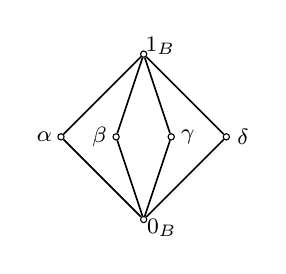
\begin{tikzpicture}[scale=.7]
                \node (250) at (2.5,0)  [draw, circle, inner sep=\dotsize] {};
        \node (253) at (2.5,3)  [draw, circle, inner sep=\dotsize] {};
        \foreach \i in {1,...,4} 
                 { 
                   \node (\i15) at (\i,1.5)  [draw, circle, inner sep=\dotsize] {};
                   \draw[semithick] (250) to (\i15) to (253);
                 }

        \draw[font=\footnotesize] 
        (0.7,1.5) node {$\alpha$} (1.7,1.5) node {$\beta$}
        (3.3,1.5) node {$\gamma$} (4.3,1.5) node {$\delta$}
        (2.8,3.15) node {$1_B$} (2.83,-.15) node {$0_B$};
      \end{tikzpicture}
    \end{column}

    \begin{column}{0.4\textwidth}
      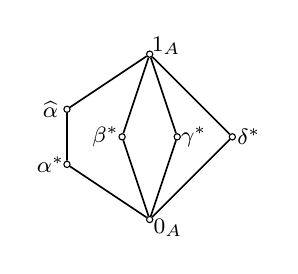
\begin{tikzpicture}[scale=.7]
              \node (70) at (6.5,0)  [draw, circle, inner sep=\dotsize] {};
      \node (71) at (7,1.5)  [draw, circle, inner sep=\dotsize] {};
      \node (73) at (6.5,3)  [draw, circle, inner sep=\dotsize] {};
      \node (61) at (6,1.5)  [draw, circle, inner sep=\dotsize] {};
      \node (51) at (5,1)  [draw, circle, inner sep=\dotsize] {};
      \node (52) at (5,2)  [draw, circle, inner sep=\dotsize] {};
      \node (81) at (8,1.5)  [draw, circle, inner sep=\dotsize] {};
      \draw[semithick] 
      (70) to (51) to (52) to (73)
      (70) to (61) to (73) 
      (70) to (71) to (73) 
      (70) to (81) to (73);

        \draw[font=\footnotesize] 
        (4.7,1) node {$\alpha^*$} (4.7,2) node {$\widehat{\alpha}$}
        (5.7,1.5) node {$\beta^*$} (7.3,1.5) node {$\gamma^*$} (8.3,1.5) node {$\delta^*$}
        (6.8,3.15) node {$1_A$} (6.83,-.15) node {$0_A$};
      \end{tikzpicture}
    \end{column}

  \end{columns}

  \begin{columns}
    \begin{column}{0.3\textwidth}
      \begin{center}
        $\Con \< B,\{g_0, g_1\}\>$

        \vskip-2pt
        \begin{align*}
          \alpha &= {\color<2->{blue}\pb 0, 1, 2 \pb 3, 4, 5\pb }\\[4pt]
          \beta &= {\color<2->{blue}\pb 0, 3 \pb  1, 4 \pb 2, 5 \pb} \\[3pt]
          \gamma &= {\color<2->{blue}\pb 0, 4\pb 1, 5\pb  2, 3\pb}  \\[3pt]
          \delta &= {\color<2->{blue}\pb 0, 5\pb 1, 3\pb  2, 4\pb} 
        \end{align*}
      \end{center}
    \end{column}

    \begin{column}{0.65\textwidth}
      \begin{center}
        $\Con \<A, F_A\>$
      \end{center}
      \begin{align*}
        \widehat{\alpha} &=|{\color<2->{blue}0,1,2},6,7,11,12|{\color<2->{blue}3,4,5}|8,9,10,13,14,15| \\
        \alpha^* &=|{\color<2->{blue}0,1,2},6,7,11,12|{\color<2->{blue}3,4,5}|8,9,10|13,14,15| \\[2pt]
        \beta^*&=|{\color<2->{blue}0,3},8|{\color<2->{blue}1,4}|{\color<2->{blue}2,5},15|6,9|7,10|11,13|12,14| \\[2pt]
        \gamma^*&=|{\color<2->{blue}0,4},9|{\color<2->{blue}1,5}|{\color<2->{blue}2,3},13|6,10|7,8|11,14|12,15| \\[2pt]
        \delta^*&=|{\color<2->{blue}0,5},10|{\color<2->{blue}1,3}|{\color<2->{blue}2,4},14|6,8|7,9,11,15|12,13|
      \end{align*}
    \end{column}
  \end{columns}

  \vskip4mm

  \only<2>{\[
    \alpha = \alpha^*\cap B^2 = \widehat{\alpha}\cap B^2,\; \quad
    \beta = \beta^*\cap B^2, \quad \dots %\quad \gamma = \gamma^*\cap B^2, \quad \delta = \delta^*\cap B^2.
    \]}

\end{frame}

\newcommand{\ifdot}{dotted}
%\newcommand{\ifdot}{dashed}
%\newcommand{\ifdot}{}

\begin{frame}[fragile,label=OA,shrink=5]{Why does it work?}
  \begin{columns}
    \begin{column}{0.3\textwidth}
      \begin{center}
        $\Con \< B,\{g_0, g_1\}\>$

        \vskip-2pt
        \begin{align*}
          \alpha &= |{\color<2,6,7>{blue}0, 1, 2} | {\color<2,6,7>{blue}3, 4, 5}|\\[4pt]
          \beta &= |{\color<3>{blue}0, 3} | {\color<3>{blue}1, 4} |{\color<3>{blue}2, 5} | \\[3pt]
          \gamma &= |{\color<4>{blue}0, 4}|{\color<4>{blue}1, 5}|{\color<4>{blue}2, 3}| \\[3pt]
          \delta &= |{\color<5>{blue}0, 5}|{\color<5>{blue}1, 3}|{\color<5>{blue} 2, 4}| 
        \end{align*}
      \end{center}
    \end{column}

    \begin{column}{0.4\textwidth}
      {
        \begin{tikzpicture}[scale=.7]

          \visible<1-48,62->{ % B_0
            \foreach \j in {0,1,2} {
              \draw (\j -1, 0.5) node {$\j$};
              \pgfmathtruncatemacro{\x}{\j+3}
              \draw (\j -1, -0.5) node {$\x$};
            }
            \draw (0,-1.5) node {$B_0$};
          }

          \visible<2,6>{ % alpha
            \draw[rounded corners,\ifdot] (-1.3,-.8) rectangle (1.3,-.2);
            \draw[rounded corners,\ifdot] (-1.3,.8) rectangle (1.3,.2);
            \draw[font=\Large] (-2,-1) node {$\alpha$};
          }
          \visible<3>{  % beta
            \draw[rounded corners,\ifdot] (-1.3,-.8) rectangle (-.7,.8);
            \draw[rounded corners,\ifdot] (-.3,-.8) rectangle (.3,.8);
            \draw[rounded corners,\ifdot] (1.3,-.8) rectangle (.7,.8);
            \draw[font=\Large] (-2,-1) node {$\beta$};
          }
          \visible<4>{   % beta
            \draw[rounded corners,\ifdot] (1,-.85) to (1.35,-.5) to  (-0,.85) to (-.35,.5) to (1,-.85);
            \draw[rounded corners,\ifdot] (0,-.85) to (0.35,-.5) to  (-1,.85) to (-1.35,.5) to (0,-.85);
            \draw[rounded corners,\ifdot] (.8,.05) to (1.37,.35) to  (1.1,.87) to (.4,.4);
            \draw[rounded corners,\ifdot] (-.8,-.05) to (-1.37,-.35) to  (-1.1,-.87) to (-.4,-.4);
            \draw[\ifdot] (-0.1,.2) to (-.28,.13);
            \draw[\ifdot] (0.1,-.2) to (.28,-.13);
            \draw[font=\Large] (-2,-1) node {$\gamma$};
          }

          \visible<5>{ % delta
            \draw[rounded corners,\ifdot] (-1,-.85) to (-1.35,-.5) to  (0,.85) to (.35,.5) to (-1,-.85);
            \draw[rounded corners,\ifdot] (0,-.85) to (-0.35,-.5) to  (1,.85) to (1.35,.5) to (0,-.85);
            \draw[rounded corners,\ifdot] (-.8,.05) to (-1.37,.35) to  (-1.1,.87) to (-.4,.4);
            \draw[rounded corners,\ifdot] (.8,-.05) to (1.37,-.35) to  (1.1,-.87) to (.4,-.4);
            \draw[\ifdot] (0.1,.2) to (.28,.13);
            \draw[\ifdot] (-0.1,-.2) to (-.28,-.13);
            \draw[font=\Large] (-2,-1) node {$\delta$};
          }

          %% B0 rectangle %%
          \visible<8-34>{\draw[rounded corners,blue] (-1.5,-1) rectangle (1.5,1); }
          \visible<1-7,35-48,62->{\draw[rounded corners,dotted] (-1.5,-1) rectangle (1.5,1);}

          %% B1 %%
          \visible<7,35->{ 
            \foreach \j in {0,1,2} {
              \pgfmathtruncatemacro{\x}{10-\j}
              \draw (\j -3, 1.5) node {$\x$};
            }
            \draw (-3, .5) node {$7$} (-2, .5) node {$6$}; 
          }
          \visible<7,8,35->{\draw  (-2,2.5) node {$B_1$};}
          \visible<7,62->{\draw[rounded corners,dotted] (-3.5,0) rectangle (-0.5,2);}
          \visible<35-61>{\draw[rounded corners,blue] (-3.5,0) rectangle (-0.5,2);}
          \visible<49-61>{\draw (-1, .5) node {$0$}; }

          %% B2 %%
          \visible<7-21,62->{ 
            {\color<9-21>{gray}
              \foreach \j in {0,1,2} {
                \pgfmathtruncatemacro{\y}{15-\j}
                \draw (\j +1, 1.5) node {$\y$};
              }
              \draw (3, .5) node {$11$} (2, .5) node {$12$};
            }
          }
          \visible<7-22,35,62->{\draw  (2,2.5) node {$B_2$};}
          \visible<7-21,62->{\draw[rounded corners,dotted] (3.5,0) rectangle (0.5,2);}

          \foreach \i in {0,...,11}{
            \pgfmathtruncatemacro{\v}{\i+8}
            \visible<\v>{ 
              {\color<18-19>{gray}
                \eImageOfBOne{\i}}
            }
          }
          \foreach \i in {0,...,11}{
            \pgfmathtruncatemacro{\v}{\i+22}
            \visible<\v>{ 
              {\color<32-33>{gray}
                \eImageOfBTwo{\i}
              }
            }
          }

          \foreach \i in {0,...,11}{
            \pgfmathtruncatemacro{\v}{\i+35}
            \visible<\v>{ 
              {\color<46-47>{gray}
                \eImageOfBTwo{\i}
              }
            }
          }

        %% Rotate B0 onto B1 %%
        \foreach \i in {0,1,...,11}{
          \pgfmathtruncatemacro{\v}{\i+49}
          \visible<\v>{ 
            {\color<60-61>{gray}
              \eImageOfBZero{\i}       %% use -\i for clockwise rotation
            }
          }
        }

        \end{tikzpicture}
      }
    \end{column}
  \end{columns}
  \begin{columns}
    \begin{column}{0.3\textwidth}
      \begin{itemize}
      \item<7-> $A = B_0 \cup B_1 \cup B_2$
        \vskip4pt
      \item<8->Unary operations 
        \begin{align*}
          \alt<8-34>{{\color{blue} e_0} & {\color{blue} : A \twoheadrightarrow B_0 }}
                    {{\color{gray} e_0} & {\color{gray} : A \twoheadrightarrow B_0 }}\\
          \alt<35-61>{{\color{blue} e_1} &{\color{blue} : A \twoheadrightarrow B_1}}
                     {{\color{gray} e_1} &{\color{gray} : A \twoheadrightarrow B_1}}\\
          {\color{gray} e_2} &{\color{gray} : A \twoheadrightarrow B_2}\\
          \alt<62>{{\color{blue} s} &{\color{blue} : A \twoheadrightarrow B_0}}
                  {{\color{gray} s} &{\color{gray} : A \twoheadrightarrow B_0}}\\
        \end{align*}
        \[
        \alt<63>{{\color{blue} g e_0} {\color{blue} : A \stackrel{e_0}{\twoheadrightarrow} B_0 \stackrel{g}{\rightarrow} B_0}}
                {{\color{gray} g e_0} {\color{gray} : A \stackrel{e_0}{\twoheadrightarrow} B_0 \stackrel{g}{\rightarrow} B_0}}
        \]
      \end{itemize}
    \end{column}
    \begin{column}{0.5\textwidth}
      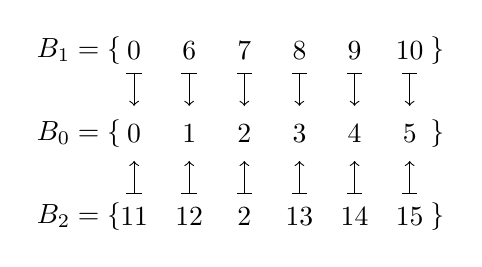
\begin{tikzpicture}[scale=.7]

        \visible<6->{                      
          
          %%% B_0 %%%
          \draw (-1,0) node {$B_0 = \{$};
          \foreach \i in { 0, 1, 2, 3, 4, 5}{ 
            \draw (\i,0) node {$\i$}; 
            \visible<8,9,12,13,16,17,20,21-34>{ \draw [|->] (\i,1.1) -- (\i,0.5);}
            \visible<8-23,26-28,31-34>{ \draw [|->] (\i,-1.1) -- (\i,-0.5); }
          }
          \draw (5.5,0) node {$\}$};
        }
        
        \visible<7->{                                               

          %%% B_1 %%%
          \draw (-1,1.5) node {$B_1 =\{$} (0,1.5) node {$0$};
          \foreach \i in { 6, 7, 8, 9, 10}{ \draw (\i-5,1.5) node {$\i$}; }
          \draw (5.5,1.5) node {$\}$};
          
          %%% B_2 %%%
          \draw (-1,-1.5) node {$B_2 =\{$} (0,-1.5) node {$11$} (1,-1.5) node {$12$} (2,-1.5) node {$2$};
          \foreach \i in { 13, 14, 15}{ \draw (\i-10,-1.5) node {$\i$}; }
          \draw (5.5,-1.5) node {$\}$};
        }

      \end{tikzpicture}
    \end{column}

  \end{columns}
\end{frame}





\begin{frame}[fragile,label=OAop3,shrink=5]{Why does it work?}

  \begin{columns}
    \begin{column}{0.3\textwidth}
      \begin{center}
        $\Con \< B,\{g_0, g_1\}\>$

        \vskip-2pt
        \begin{align*}
          \alpha &= |0, 1, 2 | 3, 4, 5|\\[4pt]
          \beta &= |0, 3 | 1, 4 |2, 5 | \\[3pt]
          \gamma &= |0, 4| 1, 5|2, 3| \\[3pt]
          \delta &= |0, 5|1, 3|2, 4| 
        \end{align*}
      \end{center}
    \end{column}

    \begin{column}{0.3\textwidth}
      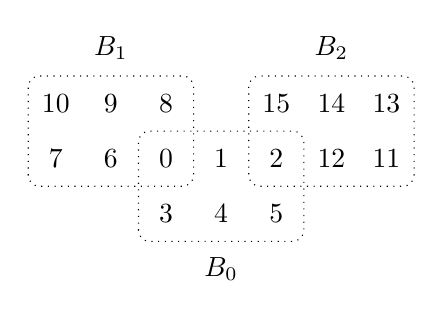
\begin{tikzpicture}[scale=.7]

        %% B0 %%
        \foreach \j in {0,1,2} {
          \draw (\j -1, 0.5) node {$\j$};
          \pgfmathtruncatemacro{\x}{\j+3}
          \draw (\j -1, -0.5) node {$\x$};
        }
        \draw (0,-1.5) node {$B_0$};
        \draw[rounded corners,dotted] (-1.5,-1) rectangle (1.5,1);

        %% B1 %%
        \foreach \j in {0,1,2} {
          \pgfmathtruncatemacro{\x}{10-\j}
          \draw (\j -3, 1.5) node {$\x$};
        }
        \draw (-3, .5) node {$7$} (-2, .5) node {$6$}; 
        \draw[rounded corners,dotted] (-3.5,0) rectangle (-0.5,2);
        \draw  (-2,2.5) node {$B_1$};

        %% B2 %%
        \foreach \j in {0,1,2} {
          \pgfmathtruncatemacro{\y}{15-\j}
          \draw (\j +1, 1.5) node {$\y$};
        }
        \draw (3, .5) node {$11$} (2, .5) node {$12$};
        \draw  (2,2.5) node {$B_2$};
        \draw[rounded corners,dotted] (3.5,0) rectangle (0.5,2);


      \end{tikzpicture}
    \end{column}
  \end{columns}
  \begin{columns}
    \begin{column}{0.3\textwidth}
      \begin{itemize}
      \item $A = B_0 \cup B_1 \cup B_2$
        \vskip4pt
      \item Unary operations 
        \begin{align*}
          {\color{gray} e_0} & {\color{gray} : A \twoheadrightarrow B_0 } \\
          {\color{gray} e_1} &{\color{gray} : A \twoheadrightarrow B_1}\\
          {\color{gray} e_2} &{\color{gray} : A \twoheadrightarrow B_2}\\
          {\color{blue} s} &{\color{blue} : A \twoheadrightarrow B_0}
        \end{align*}
        \[
          {\color{gray} g e_0} {\color{gray} : A \stackrel{e_0}{\twoheadrightarrow} B_0 \stackrel{g}{\rightarrow} B_0}
          \]
      \end{itemize}
    \end{column}
    \begin{column}{0.5\textwidth}
      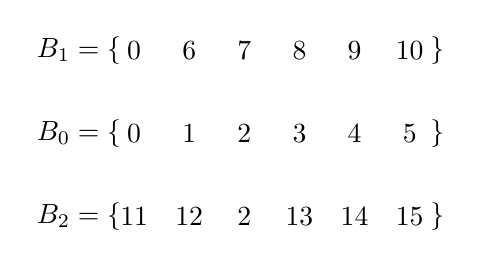
\begin{tikzpicture}[scale=.7]

        %%% B_0 %%%
        \draw (-1,0) node {$B_0 = \{$};
        \foreach \i in { 0, 1, 2, 3, 4, 5}{ 
          \draw (\i,0) node {$\i$}; 
        }
        \draw (5.5,0) node {$\}$};

        %%% B_1 %%%
        \draw (-1,1.5) node {$B_1 =\{$} (0,1.5) node {$0$};
        \foreach \i in { 6, 7, 8, 9, 10}{ \draw (\i-5,1.5) node {$\i$}; }
        \draw (5.5,1.5) node {$\}$};
        
        %%% B_2 %%%
        \draw (-1,-1.5) node {$B_2 =\{$} (0,-1.5) node {$11$} (1,-1.5) node {$12$} (2,-1.5) node {$2$};
        \foreach \i in { 13, 14, 15}{ \draw (\i-10,-1.5) node {$\i$}; }
        \draw (5.5,-1.5) node {$\}$};


      \end{tikzpicture}
    \end{column}

  \end{columns}
\end{frame}



\renewcommand{\ifdot}{dotted}
\begin{frame}[fragile,label=OAcong,shrink=5]{Why does it work?}

  \begin{columns}
    \begin{column}{0.3\textwidth}
      \begin{center}
        $\Con \< B,\{g_0, g_1\}\>$

        \vskip-2pt
        \begin{align*}
          \alpha &= {\color<2>{blue} \pb 0, 1, 2 \pb 3, 4, 5\pb }\\[4pt]
          \beta &= {\color<5>{blue} \pb 0, 3 \pb 1, 4 \pb 2, 5 \pb} \\[3pt]
          \gamma &= |0, 4| 1, 5|2, 3| \\[3pt]
          \delta &= |0, 5|1, 3|2, 4| 
        \end{align*}
      \end{center}
    \end{column}

    \begin{column}{0.3\textwidth}
      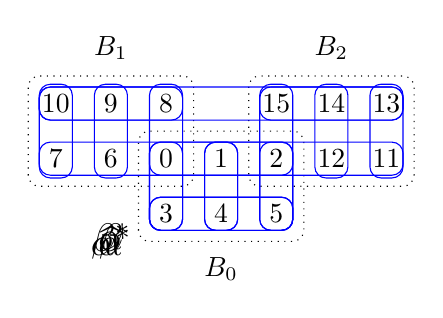
\begin{tikzpicture}[scale=.7]

        %% B0 %%
        \foreach \j in {0,1,2} {
          \draw (\j -1, 0.5) node {$\j$};
          \pgfmathtruncatemacro{\x}{\j+3}
          \draw (\j -1, -0.5) node {$\x$};
        }
        \draw (0,-1.5) node {$B_0$};
        \draw[rounded corners,dotted] (-1.5,-1) rectangle (1.5,1);

        %% B1 %%
        \foreach \j in {0,1,2} {
          \pgfmathtruncatemacro{\x}{10-\j}
          \draw (\j -3, 1.5) node {$\x$};
        }
        \draw (-3, .5) node {$7$} (-2, .5) node {$6$}; 
        \draw[rounded corners,dotted] (-3.5,0) rectangle (-0.5,2);
        \draw  (-2,2.5) node {$B_1$};

        %% B2 %%
        \foreach \j in {0,1,2} {
          \pgfmathtruncatemacro{\y}{15-\j}
          \draw (\j +1, 1.5) node {$\y$};
        }
        \draw (3, .5) node {$11$} (2, .5) node {$12$};
        \draw  (2,2.5) node {$B_2$};
        \draw[rounded corners,dotted] (3.5,0) rectangle (0.5,2);

        \visible<2>{ % alpha
          \draw[rounded corners,blue] (-1.3,-.8) rectangle (1.3,-.2);
          \draw[rounded corners,blue] (-1.3,.8) rectangle (1.3,.2);
          \draw[font=\Large] (-2,-1) node {$\alpha$};
        }
        \visible<3,4>{ % \alpha^*
          % B0 lower rectangle
          \draw[rounded corners,blue] (-1.3,-.8) rectangle (1.3,-.2);
          % long rectangle
          \draw[rounded corners,blue] (-3.3,.8) rectangle (3.3,.2); 
        }
        \visible<3>{ % \alpha^*
          \draw[rounded corners,blue] (-3.3,1.2) rectangle (-.7,1.8);  
          \draw[rounded corners,blue] (3.3,1.2) rectangle (.7,1.8); 
          \draw[font=\Large] (-2,-1) node {$\alpha^*$};
        }
        \visible<4>{ % \widehat{\alpha}
          \draw[rounded corners,blue] (-3.3,1.2) rectangle (3.3,1.8);  
          \draw[font=\Large] (-2,-1) node {$\widehat{\alpha}$};
        }
        \visible<5>{  % beta
          \draw[rounded corners,blue] (-1.3,-.8) rectangle (-.7,.8);
          \draw[rounded corners,blue] (-.3,-.8) rectangle (.3,.8);
          \draw[rounded corners,blue] (1.3,-.8) rectangle (.7,.8);
          \draw[font=\Large] (-2,-1) node {$\beta$};
        }
        \visible<6->{  % beta
          \draw[rounded corners,blue] (-1.3,-.8) rectangle (-.7,1.85);  % big left rect
          \draw[rounded corners,blue] (-.3,-.8) rectangle (.3,.8);
          \draw[rounded corners,blue] (1.3,-.8) rectangle (.7,1.85);  % big right rect
          \draw[rounded corners,blue] (-1.7,.15) rectangle (-2.3,1.85);
          \draw[rounded corners,blue] (-2.7,.15) rectangle (-3.3,1.85);  % small B1 far left
          \draw[rounded corners,blue] (1.7,.15) rectangle (2.3,1.85);
          \draw[rounded corners,blue] (2.7,.15) rectangle (3.3,1.85); % small B2 far right
          \draw[font=\Large] (-2,-1) node {$\beta^*$};
        }

      \end{tikzpicture}
    \end{column}
  \end{columns}
  \begin{columns}
    \begin{column}{0.3\textwidth}
      \visible<7>{\emph{Why don't the $\beta$ classes of $B_1$ and $B_2$ mix?}}
    \end{column}
    \begin{column}{0.5\textwidth}
      \begin{center}
        $\Con \<A, F_A\>$
      \end{center}
      \begin{align*}
        \widehat{\alpha} &= {\color<4>{blue} \pb 0,1,2,6,7,11,12\pb 3,4,5 \pb 8,9,10,13,14,15\pb } \\
        \alpha^* &= {\color<3>{blue} \pb  0,1,2,6,7,11,12 \pb 3,4,5 \pb 8,9,10 \pb 13,14,15 \pb}  \\[2pt]
        \beta^*&= {\color<6->{blue} \pb 0,3,8 \pb 1,4 \pb 2,5,15 \pb 6,9 \pb 7,10 \pb 11,13 \pb 12,14 \pb } \\[2pt]
        \gamma^*&= \pb 0,4,9 \pb 1,5 \pb 2,3,13 \pb 6,10 \pb 7,8 \pb 11,14 \pb 12,15 \pb  \\[2pt]
        \delta^*&= \pb 0,5,10 \pb 1,3 \pb 2,4,14 \pb 6,8 \pb 7,9,11,15 \pb 12,13 \pb 
      \end{align*}
    \end{column}

  \end{columns}
\end{frame}

\begin{frame}[fragile,label=OAEx2,shrink=5]{Variations on the same example... }

  \begin{columns}
    \begin{column}{0.7\textwidth}
      \begin{itemize}
      \item 
        Suppose we want $\beta = \Cg^\bB(0,3) =| 0, 3 | 2, 5 | 1, 4 |$ to 
        \vskip4pt
        have non-trivial inverse image $\beta\resB^{-1} = [\beta^*, \widehat{\beta}]$.  
        \vskip6pt
      \item<2-> Select elements 0 and 3 as intersection points:
        \[
        A = B_0 \cup B_1 \cup B_2 \quad \text{where}
        \]
        \begin{align*}
          B_0 &= \{{\color{blue} 0}, 1,  2,  {\color{green}3},  4,  5\}\\
          B_1 &= \{{\color{blue} 0}, 6,  7,  8,  9, 10\}\\
          B_2 &= \{11, 12, 13, {\color{green}3}, 14, 15\}.
        \end{align*}
      \end{itemize}
    \end{column}
    \begin{column}{0.3\textwidth}
      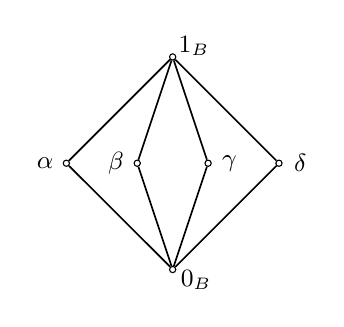
\begin{tikzpicture}[scale=.9]
                \node (250) at (2.5,0)  [draw, circle, inner sep=\dotsize] {};
        \node (253) at (2.5,3)  [draw, circle, inner sep=\dotsize] {};
        \foreach \i in {1,...,4} 
                 { 
                   \node (\i15) at (\i,1.5)  [draw, circle, inner sep=\dotsize] {};
                   \draw[semithick] (250) to (\i15) to (253);
                 }

        \draw[font=\small] 
        (0.7,1.5) node {$\alpha$} (1.7,1.5) node {$\beta$}
        (3.3,1.5) node {$\gamma$} (4.3,1.5) node {$\delta$}
        (2.8,3.15) node {$1_B$} (2.83,-.15) node {$0_B$};
      \end{tikzpicture}

    \end{column}

  \end{columns}

  \vskip-5mm

  \begin{columns}
    \begin{column}{0.3\textwidth}

      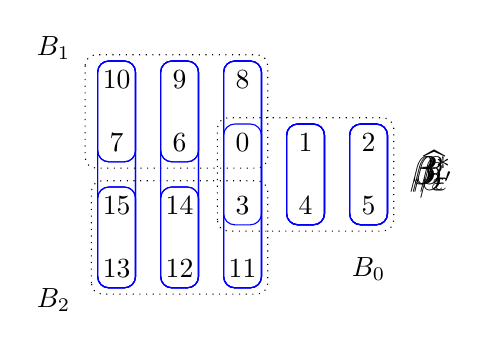
\begin{tikzpicture}[scale=.8]

        %% B0 %%
        \foreach \j in {0,1,2} {
          \draw (\j -1, 0.5) node {$\j$};
          \pgfmathtruncatemacro{\x}{\j+3}
          \draw (\j -1, -0.5) node {$\x$};
        }
        \draw (1,-1.5) node {$B_0$};
        \draw[rounded corners,dotted] (-1.4,-.9) rectangle (1.4,.9);

        \visible<3->{

          %% B1 %%
          \foreach \j in {0,1,2} {
            \pgfmathtruncatemacro{\x}{10-\j}
            \draw (\j -3, 1.5) node {$\x$};
          }
          \draw (-3, .5) node {$7$} (-2, .5) node {$6$}; 
          \draw[rounded corners,dotted] (-3.5,1.9) rectangle (-0.6,.1);
          \draw  (-4,2) node {$B_1$};

          %% B2 %%
          \foreach \j in {0,1,2} {
            \pgfmathtruncatemacro{\y}{13-\j}
            \draw (\j -3, -1.5) node {$\y$};
          }
          \draw (-3, -.5) node {$15$} (-2, -.5) node {$14$};
          \draw  (-4,-2) node {$B_2$};
          \draw[rounded corners,dotted] (-3.4,-1.9) rectangle (-0.6,-.1);
        }

        \visible<1-3>{  % beta
          \draw[rounded corners,blue] (-1.3,-.8) rectangle (-.7,.8);
          \draw[rounded corners,blue] (-.3,-.8) rectangle (.3,.8);
          \draw[rounded corners,blue] (1.3,-.8) rectangle (.7,.8);
          \draw[font=\Large] (2,0) node {$\beta$};
        }
        \visible<4>{  % beta^*
          \draw[rounded corners,blue] (-1.3,-1.8) rectangle (-.7,1.8);  % big rect
          \draw[rounded corners,blue] (-.3,-.8) rectangle (.3,.8);
          \draw[rounded corners,blue] (.7,-.8) rectangle (1.3,.8);     % right rect
          \draw[rounded corners,blue] (-1.7,.2) rectangle (-2.3,1.8);  % small B1 middle
          \draw[rounded corners,blue] (-2.7,.2) rectangle (-3.3,1.8);  % small B1 left
          \draw[rounded corners,blue] (-1.7,-.2) rectangle (-2.3,-1.8);% small B2 middle 
          \draw[rounded corners,blue] (-2.7,-.2) rectangle (-3.3,-1.8);% small B2 far left
          \draw[font=\Large] (2,0) node {$\beta^*$};
        }
        \visible<5>{  % \widehat{\beta}
          \draw[rounded corners,blue] (-1.3,-1.8) rectangle (-.7,1.8);  % big B0 rect
          \draw[rounded corners,blue] (-.3,-.8) rectangle (.3,.8);        % middle B0 rect
          \draw[rounded corners,blue] (.7,-.8) rectangle (1.3,.8);        % right B0 rect
          \draw[rounded corners,blue] (-3.3,-1.8) rectangle (-2.7,1.8);    % large far left
          \draw[rounded corners,blue] (-2.3,-1.8) rectangle (-1.7,1.8);  % small B2 far left
          \draw[font=\Large] (2,0) node {$\widehat{\beta}$};
        }
        \visible<6>{  % beta\eps1
          \draw[rounded corners,blue] (-1.3,-1.8) rectangle (-.7,1.8); % big rect
          \draw[rounded corners,blue] (-.3,-.8) rectangle (.3,.8);     % middle B0 rect
          \draw[rounded corners,blue] (.7,-.8) rectangle (1.3,.8);     % right rect
          \draw[rounded corners,blue] (-2.7,.2) rectangle (-3.3,1.8);  % small B1 left
          \draw[rounded corners,blue] (-1.7,1.8) rectangle (-2.3,-1.8);% big B1B2 middle 
          \draw[rounded corners,blue] (-2.7,-.2) rectangle (-3.3,-1.8);% small B2 far left
          \draw[font=\Large] (2,0) node {$\beta_\eps$};
        }
        \visible<7->{  % beta\eps2
          \draw[rounded corners,blue] (-1.3,-1.8) rectangle (-.7,1.8); % big rect
          \draw[rounded corners,blue] (-.3,-.8) rectangle (.3,.8);     % middle B0 rect
          \draw[rounded corners,blue] (.7,-.8) rectangle (1.3,.8);     % right rect
          \draw[rounded corners,blue] (-1.7,.2) rectangle (-2.3,1.8);  % small B1 middle
          \draw[rounded corners,blue] (-1.7,-.2) rectangle (-2.3,-1.8);% small B2 middle 
          \draw[rounded corners,blue] (-2.7,1.8) rectangle (-3.3,-1.8);%  big B1/B2 left
          \draw[font=\Large] (2,0) node {$\beta_{\eps'}$};
        }

      \end{tikzpicture}

    \end{column}

    \newcommand{\bigdotsize}{1.5pt}
    \begin{column}{0.3\textwidth}
      \centering
      \visible<4->{
        \begin{tikzpicture}[scale=1]
          \node (bottom) at (6.5,0)  [draw, circle, inner sep=\dotsize] {};  % bottom
          \node (71) at (7,1.5)  [draw, circle, inner sep=\dotsize] {};  % delta
          \node (top) at (6.5,3)  [draw, circle, inner sep=\dotsize] {}; % top
          \alt<4>{\node (61) at (6.1,1)  [fill, circle, red, inner sep=\bigdotsize] {};}  % beta^*}
                 {\node (61) at (6.1,1)  [draw, circle, inner sep=\dotsize] {};}  
                 \alt<5>{\node (62) at (6.1,2)  [fill, circle, red, inner sep=\bigdotsize] {};}  % hat{beta}
                        {\node (62) at (6.1,2)  [draw, circle, inner sep=\dotsize] {};}  % hat{beta}
                        \visible<6>{\node (63) at (5.7,1.5)  [fill, circle, red, inner sep=\bigdotsize] {};} % beta\eps
                        \visible<7->{\node (63) at (5.7,1.5)  [fill, circle, inner sep=\dotsize] {};} % beta\eps
                        \visible<7>{\node (64) at (6.5,1.5)  [fill, circle, red, inner sep=\bigdotsize] {};} % beta\eps'
                        \visible<8->{\node (64) at (6.5,1.5)  [fill, circle, inner sep=\dotsize] {};} % beta\eps'
                        \node (51) at (5,1.5)  [draw, circle, inner sep=\dotsize] {};  % alpha
                        \node (81) at (8,1.5)  [draw, circle, inner sep=\dotsize] {};
                        \draw[semithick] 
                        (bottom) to (51) to (top) to (62)
                        (bottom) to (61) 
                        (bottom) to (71) to (top) 
                        (bottom) to (81) to (top);
                        \visible<4-5>{\draw[dotted,semithick] (61) to (62);}
                        \visible<6->{\draw[semithick] (61) to (63) to (62);}
                        \visible<7->{\draw[semithick] (61) to (64) to (62);}
                        \draw (4.8,1.5) node {$\alpha^*$};
                        \draw (5.98,2.12) node {$\widehat{\beta}$};
                        \visible<6->{\draw (5.55,1.4) node {$\beta_\eps$};}
                        \visible<7->{\draw (6.65,1.3) node {$\beta_{\eps'}$};}
                        \draw (6,.8) node {$\beta^*$};
                        \draw (7.25,1.5) node {$\gamma^*$};
                        \draw (8.2,1.5) node {$\delta^*$};
                        \draw (6.7,3.15) node {$1_A$};
                        \draw (6.73,-.15) node {$0_A$};
        \end{tikzpicture}
      }
    \end{column}
  \end{columns}
\end{frame}






\begin{frame}[label=conclusion,shrink=5]{Seven element lattices: summary}
  \begin{columns}
    \begin{column}{0.2\textwidth}
      \begin{center}
        \begin{tikzpicture}[scale=.5]

          % L19
        \node (bottom) at (0,0)  [draw, circle, inner sep=\dotsize] {};
        \node (top) at (0,3)  [draw, circle, inner sep=\dotsize] {};
        \node (11) at (1,1)  [draw, circle, inner sep=\dotsize] {};
        \node (n11) at (-1,1)  [draw, circle, inner sep=\dotsize] {};
        \node (12) at (1,2)  [draw, circle, inner sep=\dotsize] {};
        \node (n12) at (-1,2)  [draw, circle, inner sep=\dotsize] {};
        \node (01) at (0,1)  [draw, circle, inner sep=\dotsize] {};

        \draw[semithick] (bottom) to (11) to (12) to (top) to (n12) to (n11) to (bottom) to (01) to (12);

          \draw (0,-1) node {$L_{19}$};
                {\color{red}\draw[font=\large] (1,-.6) node{$\text{\rlap{$\checkmark$}}$ };}
                %\draw[font=\footnotesize] (2.5,-.6) node { Jipsen};

        \end{tikzpicture}
      \end{center}
    \end{column}
    \begin{column}{0.2\textwidth}
      \begin{center}
        \begin{tikzpicture}[scale=.4]
          % L20
      \foreach \j in {0,...,4}
      {
        \node (0\j) at (0,\j)  [draw, circle, inner sep=\dotsize] {};
      }
      \node (152) at (1.5,2)  [draw, circle, inner sep=\dotsize] {};
      \node (n125) at (-1,2.5)  [draw, circle, inner sep=\dotsize] {};
      \draw[semithick] (01) to (02) to (03) to (04) to (n125) to (01) to (00) to (152) to (04);

          \draw (0,-1) node {$L_{20}$};
                {\color{red}\draw[font=\large] (1,-.6) node{$\text{\rlap{$\checkmark$}}$ };}
                %\draw[font=\footnotesize] (3,-.6) node { Jipsen};
        \end{tikzpicture}
      \end{center}
    \end{column}
  \end{columns}

  \begin{columns}
    \begin{column}{0.2\textwidth}
      \begin{center}
        \begin{tikzpicture}[scale=.4]

          
        \node (bottom) at (0,0)  [draw, circle, inner sep=\dotsize] {};
        \node (top) at (0,5)  [draw, circle, inner sep=\dotsize] {};
        \node (n115) at (-1,1.5)  [draw, circle, inner sep=\dotsize] {};
        \node (015) at (0,1.5)  [draw, circle, inner sep=\dotsize] {};
        \node (115) at (1,1.5)  [draw, circle, inner sep=\dotsize] {};
        \node (n252) at (-2.5,2)  [draw, circle, inner sep=\dotsize] {};
        \node (03) at (0,3)  [draw, circle, inner sep=\dotsize] {};
        \draw[semithick] 
        (bottom) to (n252) to (top)
        (bottom) to (n115) to (03) to (115) to
        (bottom) to (015) to (03) to (top);
       %\draw (-4.5,2.2) node {$L \cong$};



          \draw (0,-1) node {$L_{17}$};
                {\color{red}\draw[font=\large] (1,-1) node{$\text{\rlap{$\checkmark$}}$ };}

        \end{tikzpicture}
      \end{center}
    \end{column}

    \begin{column}{0.2\textwidth}
      \begin{center}
        \begin{tikzpicture}[scale=.5]

          %\newcommand{\dotsize}{1};
\node[lat] (0) at (0,0) {};
\node[lat] (1) at (-0,1) {};
\node[lat] (2) at (1,2) {};
\node[lat] (3) at (-1,2) {};
\node[lat] (4) at (-0,2) {};
\node[lat] (5) at (-0,3) {};
\node[lat] (6) at (-0,4) {};
%\draw[font=\scriptsize] (0,-.5) node {[A4, (C2 x C2 x C2 x C2) : A5]};
%\draw[font=\scriptsize] (0,-1) node {SmallGroup(960,11358) Index 80};

\draw[semithick]
(0) to (1) to (4) to (5) to (6)
(0) to (2) to (6) to (3) to (0);


          \draw (0,-.6) node {$L_{13}$};
                {\color{red}\draw[font=\large] (1,-.6) node{$\text{\rlap{$\checkmark$}}$ };}

        \end{tikzpicture}
      \end{center}
    \end{column}

    \begin{column}{0.2\textwidth}
      \begin{center}
        \begin{tikzpicture}[scale=.3]

          % L11 aka L3 
        \node (bottom) at (0,0)  [draw, circle, inner sep=\dotsize] {};
        \node (top) at (2,6)  [draw, circle, inner sep=\dotsize] {};
        \node (n22) at (-2,2)  [draw, circle, inner sep=\dotsize] {};
        \node (22) at (2,2)  [draw, circle, inner sep=\dotsize] {};
        \node (13) at (1,3)  [draw, circle, inner sep=\dotsize] {};
        \node (04) at (0,4)  [draw, circle, inner sep=\dotsize] {};
        \node (44) at (4,4)  [draw, circle, inner sep=\dotsize] {};

        \draw[semithick] (bottom) to (22) to (44) to (top) to (04) to (13) to (22)
        (bottom) to (n22) to (04);
  \draw (1,-1) node {$L_{11}$};
                {\color{red}\draw[font=\large] (2.3,-1) node { $\text{\rlap{$\checkmark$}}$};}

        \end{tikzpicture}
      \end{center}
    \end{column}

  \end{columns}


  \begin{columns}

    \begin{column}{0.2\textwidth}
      \begin{center}
        \begin{tikzpicture}[scale=.5]

          %% ``L9'' is the pentegon with two extra wings.
      \foreach \j in {0,3} 
      { \node (7\j) at (6.5,\j)  [draw, circle, inner sep=\dotsize] {};}
      \node (71) at (7,1.5)  [draw, circle, inner sep=\dotsize] {};
      \node (61) at (6,1.5)  [draw, circle, inner sep=\dotsize] {};
      \node (51) at (5,1.5)  [draw, circle, inner sep=\dotsize] {};
      \foreach \j in {1,2} 
      { \node (8\j) at (7.8,\j)  [draw, circle, inner sep=\dotsize] {};}
      \draw[semithick] (70) to (51) to (73) to (61) to (70) to (71) to (73) to
      (82) to (81) to (70);
      

          \draw (6.5,-1) node {$L_{9}$};
            {\color{red}\draw[font=\large] (7.5,-.6) node{$\text{\rlap{$\checkmark$}}$ };}
            %\draw[font=\large] (9.3,-.6) node { {\footnotesize Freese}};
        \end{tikzpicture}
      \end{center}
    \end{column}


    \begin{column}{0.2\textwidth}
      \begin{center}
        \begin{tikzpicture}[scale=.5]

          %%  The elusive winged-2x3 %%
      \node (01) at (0,1)  [draw, circle, inner sep=\dotsize] {};
      \foreach \j in {0,2} 
      { \node (1\j) at (1,\j)  [draw, circle, inner sep=\dotsize] {};}

      \foreach \j in {1,3} 
      { \node (2\j) at (2,\j)  [draw, circle, inner sep=\dotsize] {};}
      { \node (32) at (3,2)  [draw, circle, inner sep=\dotsize] {};}
      \draw[semithick] (10) to (01) to (12) to (23) to (32) to (21) to (10) (21) to (12);
      { \node (m11) at (-1,1)  [draw, circle, inner sep=\dotsize] {};}
      \draw[semithick] (10) to (m11) to (23);



          \visible<2>{\node (18) at (1,1.3)  [draw, circle, red, inner sep=25pt] {};}

          \draw (1,-.8) node {$L_7$};
        \end{tikzpicture}
      \end{center}
    \end{column}
  \end{columns}
\end{frame}

%% \frame[label=MO,shrink=5]{
%%   \frametitle{Has anyone seen this lattice?}
%%   \begin{center}
%%     \includegraphics[height=2.8in]{MOquestion201204}
%%   \end{center}
%% }  

\begin{frame}[fragile,label=Conclusion,shrink=5]{The exceptional seven element lattice}
  \frametitle{Interval enforceable properties}
  \begin{columns}
    \begin{column}{0.7\textwidth}
      \begin{itemize}
      %% \item  $L_7$ cannot be obtained using the overalgebra construction.
      %%   \vskip2mm
      \item<1-> A minimal representation of $L_7$ must come from a transitive $G$-set.
        \vskip2mm
      \item<2-> Suppose $L_7 \cong \lb H, G \rb$ for some finite groups $H<G$.\\[4pt]
        What can we say about the group $G$?
        \vskip2mm
      \item<3-> If we prove $G$ must have certain properties, then \FLRP\ has a
        positive answer iff every finite lattice is an interval
        in the subgroup lattice of a group \emph{satisfying all of these properties}.
        \note{
          \begin{itemize}
          \item Define $\core_G(H)$.  It is the largest normal subgroup in $G$
          contained in $H$.  It is also the kernel of the action of $G$ on the
          cosets of $H$.  
        \item $L_7 \cong \lb H, G \rb$, assume WLOG $H$ is \alert{core-free} in $G$.\\  
          Otherwise $L_7\cong \lb G/\core_G(H), H/\core_G(H) \rb$, and $H/\core_G(H)$ c.f. in $G/\core_G(H)$.
          \end{itemize}
        }
      \end{itemize}
    \end{column}
    \begin{column}{0.2\textwidth}
      \begin{center}
        \begin{tikzpicture}[scale=.5]
          %%  The elusive winged-2x3 %%
      \node (01) at (0,1)  [draw, circle, inner sep=\dotsize] {};
      \foreach \j in {0,2} 
      { \node (1\j) at (1,\j)  [draw, circle, inner sep=\dotsize] {};}

      \foreach \j in {1,3} 
      { \node (2\j) at (2,\j)  [draw, circle, inner sep=\dotsize] {};}
      { \node (32) at (3,2)  [draw, circle, inner sep=\dotsize] {};}
      \draw[semithick] (10) to (01) to (12) to (23) to (32) to (21) to (10) (21) to (12);
      { \node (m11) at (-1,1)  [draw, circle, inner sep=\dotsize] {};}
      \draw[semithick] (10) to (m11) to (23);


          \alt<1>{\draw (1,-.8) node {$L_7$};}{\draw (1,-.6) node {$H$};}
          \uncover<2->{\draw (2,3.6) node {$G$};}
        \end{tikzpicture}
      \end{center}
    \end{column}
  \end{columns}

  \only<4->{
\begin{block}{Proposition}
      \label{thm:except-seven-elem}
      Suppose $H<G$, \hskip2mm $\core_G(H) = 1$, \hskip2mm $L_7 \cong \lb H,G \rb$.
      \begin{enumerate}[(i)]
      \item<4-> $G$ is a primitive permutation group.
      \item<4-> If $N\ssubnormal G$, then $C_G(N) = 1$.
      \item<4-> $G$ contains no non-trivial abelian normal subgroup.
      \item<4-> $G$ is not solvable.
      \item<4-> $G$ is subdirectly irreducible.
      \item<4-> With the possible exception of at most one maximal subgroup, %, $M_1$ or $M_2$,
        all proper subgroups in the interval $\lb H,G \rb$ are core-free. 
      \end{enumerate}
    \end{block}
  }
  \note{  It is obvious that 
    \begin{itemize}
    \item (ii) $\Rightarrow$ (iii) $\Rightarrow$ (iv), and  
    \item (ii) $\Rightarrow$ (v), but we include these for
      emphasis;
    \item the hard work is in proving (ii) and (vi), but
      the main goal is the pair of restrictions (iii) and (v), which allow us to rule
      out a number of the O'Nan-Scott types describing primitive permutation
      groups. 
  \end{itemize}}
\end{frame}

\frame[label=milestones]{
    \frametitle{Open Problems}

\begin{enumerate}[1.]
\item
\label{item:1} Are homomorphic images of representable lattices representable?

\bigskip

\item
\label{item:2} Are subdirect products of representable lattices representable?

\bigskip

\item\label{item:3} Does representable imply ``group representable?''  \\[4pt]
{\small i.e., is the congruence lattice of a finite algebra isomorphic to an interval in the subgroup lattice of a finite group?}

\bigskip
%% \item For which $n$ is $M_n$ a congruence lattice of a finite algebra?
%% \item\label{item:4} Suppose $L$ is group representable.\\[4pt]
%% Is the filter+ideal lattice $\tilde{L} = \alpha^\uparrow \cup \beta^\downarrow$ group representable, for all $\alpha, \beta \in L$.

%% \bigskip

\item\label{item:5} Is the class of representable lattices recursive?

\end{enumerate}
}

%% \frame[label=milestones]{
%%     \frametitle{Remarks on the problems}
%% \begin{theorem}[Lucchini, 1994] The lattice $M_n$ occurs as an interval in a subgroup lattices of a finite group when
%% \[
%% n = q + 2 \qquad \text{ or } \qquad n =
%% \frac{q^t + 1}{q + 1}+ 1,\]
%% where $q$ is a prime power and $t$ is an odd prime.
%% \end{theorem}
%% At present the smallest cases for which no occurrence of $M_n$ is known are $n = 16,
%% 23, 35, \dots$.
%% }

\frame[label=milestones]{
    \frametitle{Remarks on the problems}
    \begin{itemize}
    \item 
Are homomorphic images of representable lattices representable?
\\[4pt]
If $L = \Con \<A, F\>$ and $\tilde{L}$ is the homomorphic image $\{\theta \cap B^2 \mid \theta \in L\}$, where $B = e(A)$ for some operation $e^2 = e \in F$, then $\tilde{L}=\Con \<B, F\!\mid_B\>$ .

\bigskip
\uncover<2->{
\item 
Is the class of representable lattices recursive?
\\[4pt]
In other words, is the membership problem for this class decidable?
`\\[4pt]
(Note that the class is recursively enumerable by the closure method.)
\\[4pt]
\uncover<3->{
This question asks whether it's possible to write a program that, when given a finite lattice $L$, halts with output True if $L$ is representable and False otherwise.
\\[4pt]

A negative answer would solve the finite lattice representation problem.}
}
    \end{itemize}
}

\begin{frame}[fragile]
    \frametitle{Open Problems}
One approach: try to find a computable function $f$ such that, if $L$ is a representable lattice of size $n$, then $L$ is representable as the congruence lattice of an algebra of cardinality $f(n)$ or smaller.
\\[8pt]
%% which takes as input a representable finite lattice $L$, and outputs a number $f(L)$ such that $L$ is representable as a congruence lattice on an algebra of size at most $f(L)$.

This would answer the decidability question, as follows:
\begin{small}
\begin{verbatim}
IsRepresentable( L ) {

    n:= Size( L )
    N:= f( n )

    for each L' in Sub[Eq(N)] {

        if ( L' isomorphic to L ) and ( L' is closed ):
            return True

    }

    return False

}
\end{verbatim}
\end{small}
\end{frame}


\begin{frame}[fragile,label=plug]{{\footnotesize  <advertisement> }}
  \begin{center}
\alert{Workshop on Computational Universal Algebra}
\vskip3mm
Friday, October 4, 2013
\vskip3mm
University of Louisville, KY
\vskip3mm
\large{{\tt universalalgebra.wordpress.com}}
%% \vskip4mm
%% \includegraphics[width=12cm]{WorkshopPlug}%
  \end{center}
\end{frame}




\end{document}






















\begin{frame}[fragile,label=freeseOLD,shrink=5]{Contruction of an algebra $\bA$ with $\Con \bA \cong L_9$.}

  \begin{columns}
    \begin{column}{0.2\textwidth}

      \centering
      \begin{tikzpicture}[scale=.7]
                \node (250) at (2.5,0)  [draw, circle, inner sep=\dotsize] {};
        \node (253) at (2.5,3)  [draw, circle, inner sep=\dotsize] {};
        \foreach \i in {1,...,4} 
                 { 
                   \node (\i15) at (\i,1.5)  [draw, circle, inner sep=\dotsize] {};
                   \draw[semithick] (250) to (\i15) to (253);
                 }

        \uncover<2->{
          \draw[font=\footnotesize] 
          (0.7,1.5) node {$\alpha$} (1.7,1.5) node {$\beta$}
          (3.3,1.5) node {$\gamma$} (4.3,1.5) node {$\delta$}
          (2.8,3.15) node {$1_B$} (2.83,-.15) node {$0_B$};
        }
        \visible<1>{
          \draw  (1,0) node {$M_4$};}
        \visible<2->{
          \draw  (1,0) node {$\Con \bB$};}
      \end{tikzpicture}
    \end{column}
    \begin{column}{0.8\textwidth}
      \begin{enumerate}[Step 1]
      \item<2-> 
        Take a permutational algebra $\bB = \<B, F\>$ with congruence lattice $\Con\bB \cong M_4$.

        \vskip6pt
        
        \note{There are infinitely many, but apart from those involving 
          $S_3$, $C_3 \times C_3$, and $(C_3 \times C_3) \rtimes C_3$, they are quite
          large.  The next smallest G-set with $M_4$ congruence lattice that we
          know of comes from the group 
          $G = [ ( (C_3 \times C_3) \rtimes C_2 ) \times ( (C_3 \times C_3) \rtimes C_2 ) ] \rtimes C_2$
          acting on right cosets of $H \cong D_8$.  The index in this case is $|G:H| = 81$.
          (In \GAP, {\tt G:=SmallGroup(648,725)}.)}

        {\small
          \onslide<4->{\underline{Example:}}
          \vskip4pt
%          \begin{itemize}
          \begin{itemize}[label=$\cdot$]
          \item<4->
            Let $B = \{0, 1, \dots, 5\}$ index the elements of $S_3$ and
            consider the right regular action of $S_3$ on itself.
            \vskip5pt
          \item<4->
            $g_0 = (0,4)(1,3)(2,5)$ and $g_1 = (0,1,2)(3,4,5)$ generate this
            action group, the image of $S_3 \hookrightarrow S_6$.
            \vskip5pt
          \item<4-> $\Con \<B , \{g_0, g_1\}\> \cong M_4$ with congruences
\vskip1pt
\[
\hskip-3mm            \alpha = | 0 1 2 | 3 4 5|, \; \beta = | 0 3 | 1 4 | 2 5 |, 
            \gamma = | 0 4|1 5| 2 3| , \; \delta = | 0 5|1 3| 2 4| .
            \]
          \end{itemize}
        }
      \end{enumerate}


    \end{column}
  \end{columns}

  \vskip-2mm

  \begin{columns}

    \begin{column}{0.2\textwidth}
      \begin{center}
        \begin{tikzpicture}[scale=.7]

                \node (70) at (6.5,0)  [draw, circle, inner sep=\dotsize] {};
      \node (71) at (7,1.5)  [draw, circle, inner sep=\dotsize] {};
      \node (73) at (6.5,3)  [draw, circle, inner sep=\dotsize] {};
      \node (61) at (6,1.5)  [draw, circle, inner sep=\dotsize] {};
      \node (51) at (5,1)  [draw, circle, inner sep=\dotsize] {};
      \node (52) at (5,2)  [draw, circle, inner sep=\dotsize] {};
      \node (81) at (8,1.5)  [draw, circle, inner sep=\dotsize] {};
      \draw[semithick] 
      (70) to (51) to (52) to (73)
      (70) to (61) to (73) 
      (70) to (71) to (73) 
      (70) to (81) to (73);

          \visible<1,2>{\draw  (5,0) node {$L_{9}$};}
          \visible<3->{\draw  (5,0) node {$\Con \bA$};}
          \visible<3->{\draw[font=\footnotesize] (4.7,2) node {$\widehat{\alpha}$} (4.7,1) node {$\alpha^*$};}

        \end{tikzpicture}
      \end{center}
    \end{column}
    \begin{column}{0.75\textwidth}

      \begin{itemize}
      \item<3-> {\rmfamily \emph{Goal: expand $\bB$ to an algebra $\bA$ that has
          $\alpha$ ``doubled'' in $\Con\bA$.}}
        \vskip4pt
%            {\small
              \onslide<5->{\underline{Example:}\hskip8pt $\alpha = \Cg^\bB(0,2)$. }
              \vskip4pt
%              \begin{itemize}[label=$*$]
%                \begin{enumerate}
            \item<5->[Step 2] Let $A = B_0 \cup B_1 \cup B_2$ where
              \vskip-6pt
              \begin{align*}
                B_0 &= \{ {\color<5>{blue}0}, 1, {\color<5>{green}2}, 3, 4, 5\} = B\\
                B_1 &= \{{\color<5>{blue}0}, 6, 7, 8, 9, 10\}\\
                B_2 &= \{ 11, 12, {\color<5>{green}2}, 13, 14, 15\}.
              \end{align*}
            \item<5->[Step 3] Define unary operations $e_0, e_1, e_2,\, s, \,g_0 e_0$, and $g_1 e_0$.
%                \end{enumerate}
%              \end{itemize}
%            }
      \end{itemize}
    \end{column}

  \end{columns}

\end{frame}


















\begin{frame}[fragile,label=OAopOLD,shrink=5]{Why does it work?}

  \begin{columns}
    \begin{column}{0.3\textwidth}
      \begin{center}
        $\Con \< B,\{g_0, g_1\}\>$

        \vskip-2pt
        \begin{align*}
          \alpha &= |0, 1, 2 | 3, 4, 5|\\[4pt]
          \beta &= |0, 3 | 1, 4 |2, 5 | \\[3pt]
          \gamma &= |0, 4| 1, 5|2, 3| \\[3pt]
          \delta &= |0, 5|1, 3|2, 4| 
        \end{align*}
      \end{center}
    \end{column}

    \begin{column}{0.3\textwidth}
      \begin{tikzpicture}[scale=.7]

        %% B0 %%
        \visible<1-13>{
          \foreach \j in {0,1,2} {
            \draw (\j -1, 0.5) node {$\j$};
            \pgfmathtruncatemacro{\x}{\j+3}
            \draw (\j -1, -0.5) node {$\x$};
          }
          \draw (0,-1.5) node {$B_0$};
          \draw[rounded corners,dotted] (-1.5,-1) rectangle (1.5,1);
        }
        \visible<12->{\draw (-1, 0.5) node {$0$};}

        %% B1 %%
        \foreach \j in {0,1,2} {
          \pgfmathtruncatemacro{\x}{10-\j}
          \draw (\j -3, 1.5) node {$\x$};
        }
        \draw (-3, .5) node {$7$} (-2, .5) node {$6$}; 
        \draw[rounded corners,blue] (-3.5,0) rectangle (-0.5,2);
        \draw  (-2,2.5) node {$B_1$};

        %% B2 %%
        \visible<1>{ 
          \foreach \j in {0,1,2} {
            \pgfmathtruncatemacro{\y}{15-\j}
            \draw (\j +1, 1.5) node {$\y$};
          }
          \draw (3, .5) node {$11$} (2, .5) node {$12$};
          \draw  (2,2.5) node {$B_2$};
          \draw[rounded corners,dotted] (3.5,0) rectangle (0.5,2);
        }

        %% Rotate B2 onto B0 %%
        \foreach \i in {0,1,...,11}{   
          \pgfmathtruncatemacro{\v}{\i+1}
          \visible<\v>{ 
            {\color<11-12>{gray}
              \eImageOfBTwo{\i} 
            }
          }
        }

        %% Rotate B0 onto B1 %%
        \foreach \i in {0,1,...,11}{
          \pgfmathtruncatemacro{\v}{\i+13}
          \visible<\v>{ 
            {\color<22-24>{gray}
              \eImageOfBZero{\i}       %% use -\i for clockwise rotation
            }
          }
        }

      \end{tikzpicture}
    \end{column}
  \end{columns}
  \begin{columns}
    \begin{column}{0.3\textwidth}
      \begin{itemize}
      \item $A = B_0 \cup B_1 \cup B_2$
        \vskip4pt
      \item Unary operations 
        \begin{align*}
          {\color{gray} e_0} & {\color{gray} : A \twoheadrightarrow B_0 } \\
          {\color{blue} e_1} &{\color{blue} : A \twoheadrightarrow B_1}\\
          {\color{gray} e_2} &{\color{gray} : A \twoheadrightarrow B_2}\\
          {\color{gray} s} &{\color{gray} : A \twoheadrightarrow B_0}
        \end{align*}
        \[
          {\color{gray} g e_0} {\color{gray} : A \stackrel{e_0}{\twoheadrightarrow} B_0 \stackrel{g}{\rightarrow} B_0}
          \]
      \end{itemize}
    \end{column}
    \begin{column}{0.5\textwidth}
      \begin{tikzpicture}[scale=.7]

        %%% B_0 %%%
        \draw (-1,0) node {$B_0 = \{$};
        \foreach \i in { 0, 1, 2, 3, 4, 5}{ 
          \draw (\i,0) node {$\i$}; 
          \visible<14-16,19-21,24-26>{ \draw [|->] (\i,0.5) -- (\i,1.1) ; }
          \visible<2-4,7-9,12>{ \draw [|->] (\i,-1.1) -- (\i,-0.5); }
        }
        \draw (5.5,0) node {$\}$};

        %%% B_1 %%%
        \draw (-1,1.5) node {$B_1 =\{$} (0,1.5) node {$0$};
        \foreach \i in { 6, 7, 8, 9, 10}{ \draw (\i-5,1.5) node {$\i$}; }
        \draw (5.5,1.5) node {$\}$};
        
        %%% B_2 %%%
        \draw (-1,-1.5) node {$B_2 =\{$} (0,-1.5) node {$11$} (1,-1.5) node {$12$} (2,-1.5) node {$2$};
        \foreach \i in { 13, 14, 15}{ \draw (\i-10,-1.5) node {$\i$}; }
        \draw (5.5,-1.5) node {$\}$};


      \end{tikzpicture}
    \end{column}

  \end{columns}
\end{frame}


















\begin{frame}[fragile,label=OAop4,shrink=5]{Why does it work?}

  \begin{columns}
    \begin{column}{0.3\textwidth}
      \begin{center}
        $\Con \< B,\{g_0, g_1\}\>$

        \vskip-2pt
        \begin{align*}
          \alpha &= |0, 1, 2 | 3, 4, 5|\\[4pt]
          \beta &= |0, 3 | 1, 4 |2, 5 | \\[3pt]
          \gamma &= |0, 4| 1, 5|2, 3| \\[3pt]
          \delta &= |0, 5|1, 3|2, 4| 
        \end{align*}
      \end{center}
    \end{column}

    \begin{column}{0.3\textwidth}
      \begin{tikzpicture}[scale=.7]

        %% B0 %%
        \foreach \j in {0,1,2} {
          \draw (\j -1, 0.5) node {$\j$};
          \pgfmathtruncatemacro{\x}{\j+3}
          \draw (\j -1, -0.5) node {$\x$};
        }
        \draw (0,-1.5) node {$B_0$};
        \draw[rounded corners,dotted] (-1.5,-1) rectangle (1.5,1);

        %% B1 %%
        \foreach \j in {0,1,2} {
          \pgfmathtruncatemacro{\x}{10-\j}
          \draw (\j -3, 1.5) node {$\x$};
        }
        \draw (-3, .5) node {$7$} (-2, .5) node {$6$}; 
        \draw[rounded corners,dotted] (-3.5,0) rectangle (-0.5,2);
        \draw  (-2,2.5) node {$B_1$};

        %% B2 %%
        \foreach \j in {0,1,2} {
          \pgfmathtruncatemacro{\y}{15-\j}
          \draw (\j +1, 1.5) node {$\y$};
        }
        \draw (3, .5) node {$11$} (2, .5) node {$12$};
        \draw  (2,2.5) node {$B_2$};
        \draw[rounded corners,dotted] (3.5,0) rectangle (0.5,2);


      \end{tikzpicture}
    \end{column}
  \end{columns}
  \begin{columns}
    \begin{column}{0.3\textwidth}
      \begin{itemize}
      \item $A = B_0 \cup B_1 \cup B_2$
        \vskip4pt
      \item Unary operations 
        \begin{align*}
          {\color{gray} e_0} & {\color{gray} : A \twoheadrightarrow B_0 } \\
          {\color{gray} e_1} &{\color{gray} : A \twoheadrightarrow B_1}\\
          {\color{gray} e_2} &{\color{gray} : A \twoheadrightarrow B_2}\\
          {\color{gray} s} &{\color{gray} : A \twoheadrightarrow B_0}
        \end{align*}
        \[
          {\color{blue} g e_0} {\color{blue} : A \stackrel{e_0}{\twoheadrightarrow} B_0 \stackrel{g}{\rightarrow} B_0}
          \]
      \end{itemize}
    \end{column}
    \begin{column}{0.5\textwidth}
      \begin{tikzpicture}[scale=.7]

        %%% B_0 %%%
        \draw (-1,0) node {$B_0 = \{$};
        \foreach \i in { 0, 1, 2, 3, 4, 5}{ 
          \draw (\i,0) node {$\i$}; 
        }
        \draw (5.5,0) node {$\}$};

        %%% B_1 %%%
        \draw (-1,1.5) node {$B_1 =\{$} (0,1.5) node {$0$};
        \foreach \i in { 6, 7, 8, 9, 10}{ \draw (\i-5,1.5) node {$\i$}; }
        \draw (5.5,1.5) node {$\}$};
        
        %%% B_2 %%%
        \draw (-1,-1.5) node {$B_2 =\{$} (0,-1.5) node {$11$} (1,-1.5) node {$12$} (2,-1.5) node {$2$};
        \foreach \i in { 13, 14, 15}{ \draw (\i-10,-1.5) node {$\i$}; }
        \draw (5.5,-1.5) node {$\}$};


      \end{tikzpicture}
    \end{column}

  \end{columns}
\end{frame}

